%%%%%%%%%%%%%%%%%%%%%%%% HAUB.tex %%%%%%%%%%%%%%%%%%%%%%%
%
% Root file for: Software Team Leaders Handbook (D. Hyland-Wood) March 2016
%
%%%%%%%%%%%%%%%%%%%%%%%%%%%%%%%%%%%%%%%%%%%%%%%%%%%%

%\documentclass[10pt]{book} % 10 point font
%\documentclass[11pt]{book} % 11 point font
\documentclass[12pt]{book} % 12 point font
\usepackage[a4paper, top=3cm, bottom=3cm]{geometry}
\usepackage[utf8]{inputenc}
%\usepackage[latin1]{inputenc}
\usepackage{setspace}
\usepackage{fancyhdr}
\usepackage{tocloft}
\usepackage{fancybox}

% Extension Packages
%-------------------------------------------------------------------------------
\usepackage{mathptmx}	% selects Times Roman as basic font
\usepackage{helvet}		% selects Helvetica as sans-serif font
\usepackage{courier}	% selects Courier as typewriter font
%\usepackage{type1cm}	% activate if the above 3 fonts are 
					% not available on your system
					
\usepackage{titling}
\newcommand{\subtitle}[1]{%
  \posttitle{%
    \par\end{center}
    \begin{center}\large#1\end{center}
    \vskip0.5em}%
}

\newenvironment{dedication}
    {\vspace{6ex}\begin{quotation}\begin{center}\begin{em}}
    {\par\end{em}\end{center}\end{quotation}}
    
\usepackage{makeidx}	% allows index generation
\usepackage{graphicx}	% standard LaTeX graphics tool
					% when including figure files
\usepackage{multicol}	% used for the two-column index
\usepackage[bottom]{footmisc}% places footnotes at page bottom

%\usepackage{url}		% Avoid problems with special characters in URLs
\PassOptionsToPackage{hyphens}{url}
\usepackage{hyperref}
\usepackage{breakurl}	% Apparently cannot be used when processing with pdflatex.

\usepackage{soul}		% Allow line breaks in underlined text.

\usepackage{listings}
\lstset{basicstyle=\small, columns=fixed}

\usepackage{amsmath}

\usepackage[titletoc]{appendix} % for appendices

% Fix hyphenation
\tolerance=700
\setlength{\emergencystretch}{3em}

% For layout of poetry
\usepackage{lettrine}
\usepackage{parselines}
\usepackage{xcolor}
%\definecolorseries{verso}{rgb}{last}{blue!40!black}{magenta!40!black}
\definecolorseries{verso}{rgb}{last}{black}{black}
\resetcolorseries[30]{verso}
\newenvironment{verso}{\pagebreak[3]\begin{parse lines}[\parindent=1em\noindent]{\color{verso!!+}\hspace{\row\parindent}##1\newline\color{black}}}%
{\end{parse lines}}

%\usepackage{tocbibind}	% Allows the bibliography to appear in the TOC.

\makeindex			% used for the subject index
					% NB: Springer uses the style svind.ist with the makeindex program. 
					% TODO: Should I?

% Use a single bibliography style
%\usepackage[super]{natbib} % Makes citations superscript, which is nicer but conflicts with footnotes. TODO: Change somehow.
\bibliographystyle{plain}

% Custom
%-------------------------------------------------------------------------------
\usepackage[T1]{fontenc}   % Allows words with accented characters to be cut-and-pasted, and hyphenated.
\usepackage{enumitem}
\usepackage{phonetic}

% For title page
\newcommand{\HRule}{\rule{\linewidth}{0.5mm}}
\usepackage[export]{adjustbox}

% For Russian (Cyrillic) names in endnotes:
\newcommand{\cyrrm}{\fontencoding{OT2}\selectfont\textcyrup} % cyrrm = "Roman", or really upright, normal font

\lstset{
      basicstyle = \scriptsize \ttfamily,%
      keywordstyle = [1]\bfseries\color{darkgreen},%
      stringstyle  = \ttfamily\color{darkred},%
      commentstyle = \itshape\color{darkblue},%
      showstringspaces = false,%
%     fancyvrb = true,%
      firstnumber = auto, stepnumber=1, numbersep=5pt,%
      numbers=left, numberstyle=\tiny \ttfamily,
      frame = shadowbox, frameround = ffff, rulesepcolor = \color{shadecolor},
      breaklines=true, breakatwhitespace=true,%
%      prebreak=\textellipsis,postbreak=\textellipsis,%
      emphstyle = \color{red}\underbar, emphstyle = {[2]\color{blue}\underbar},%
      extendedchars = true, inputencoding = utf8,%
%     backgroundcolor=\color{shadecolor},
      xleftmargin=5pt, xrightmargin=2pt,
      captionpos = b
}
% End Custom
%-------------------------------------------------------------------------------

\begin{document}


% Graphical Cover
%-------------------------------------------------------------------------------
\begin{titlepage}

\begin{figure}[htbp]
\begin{center}
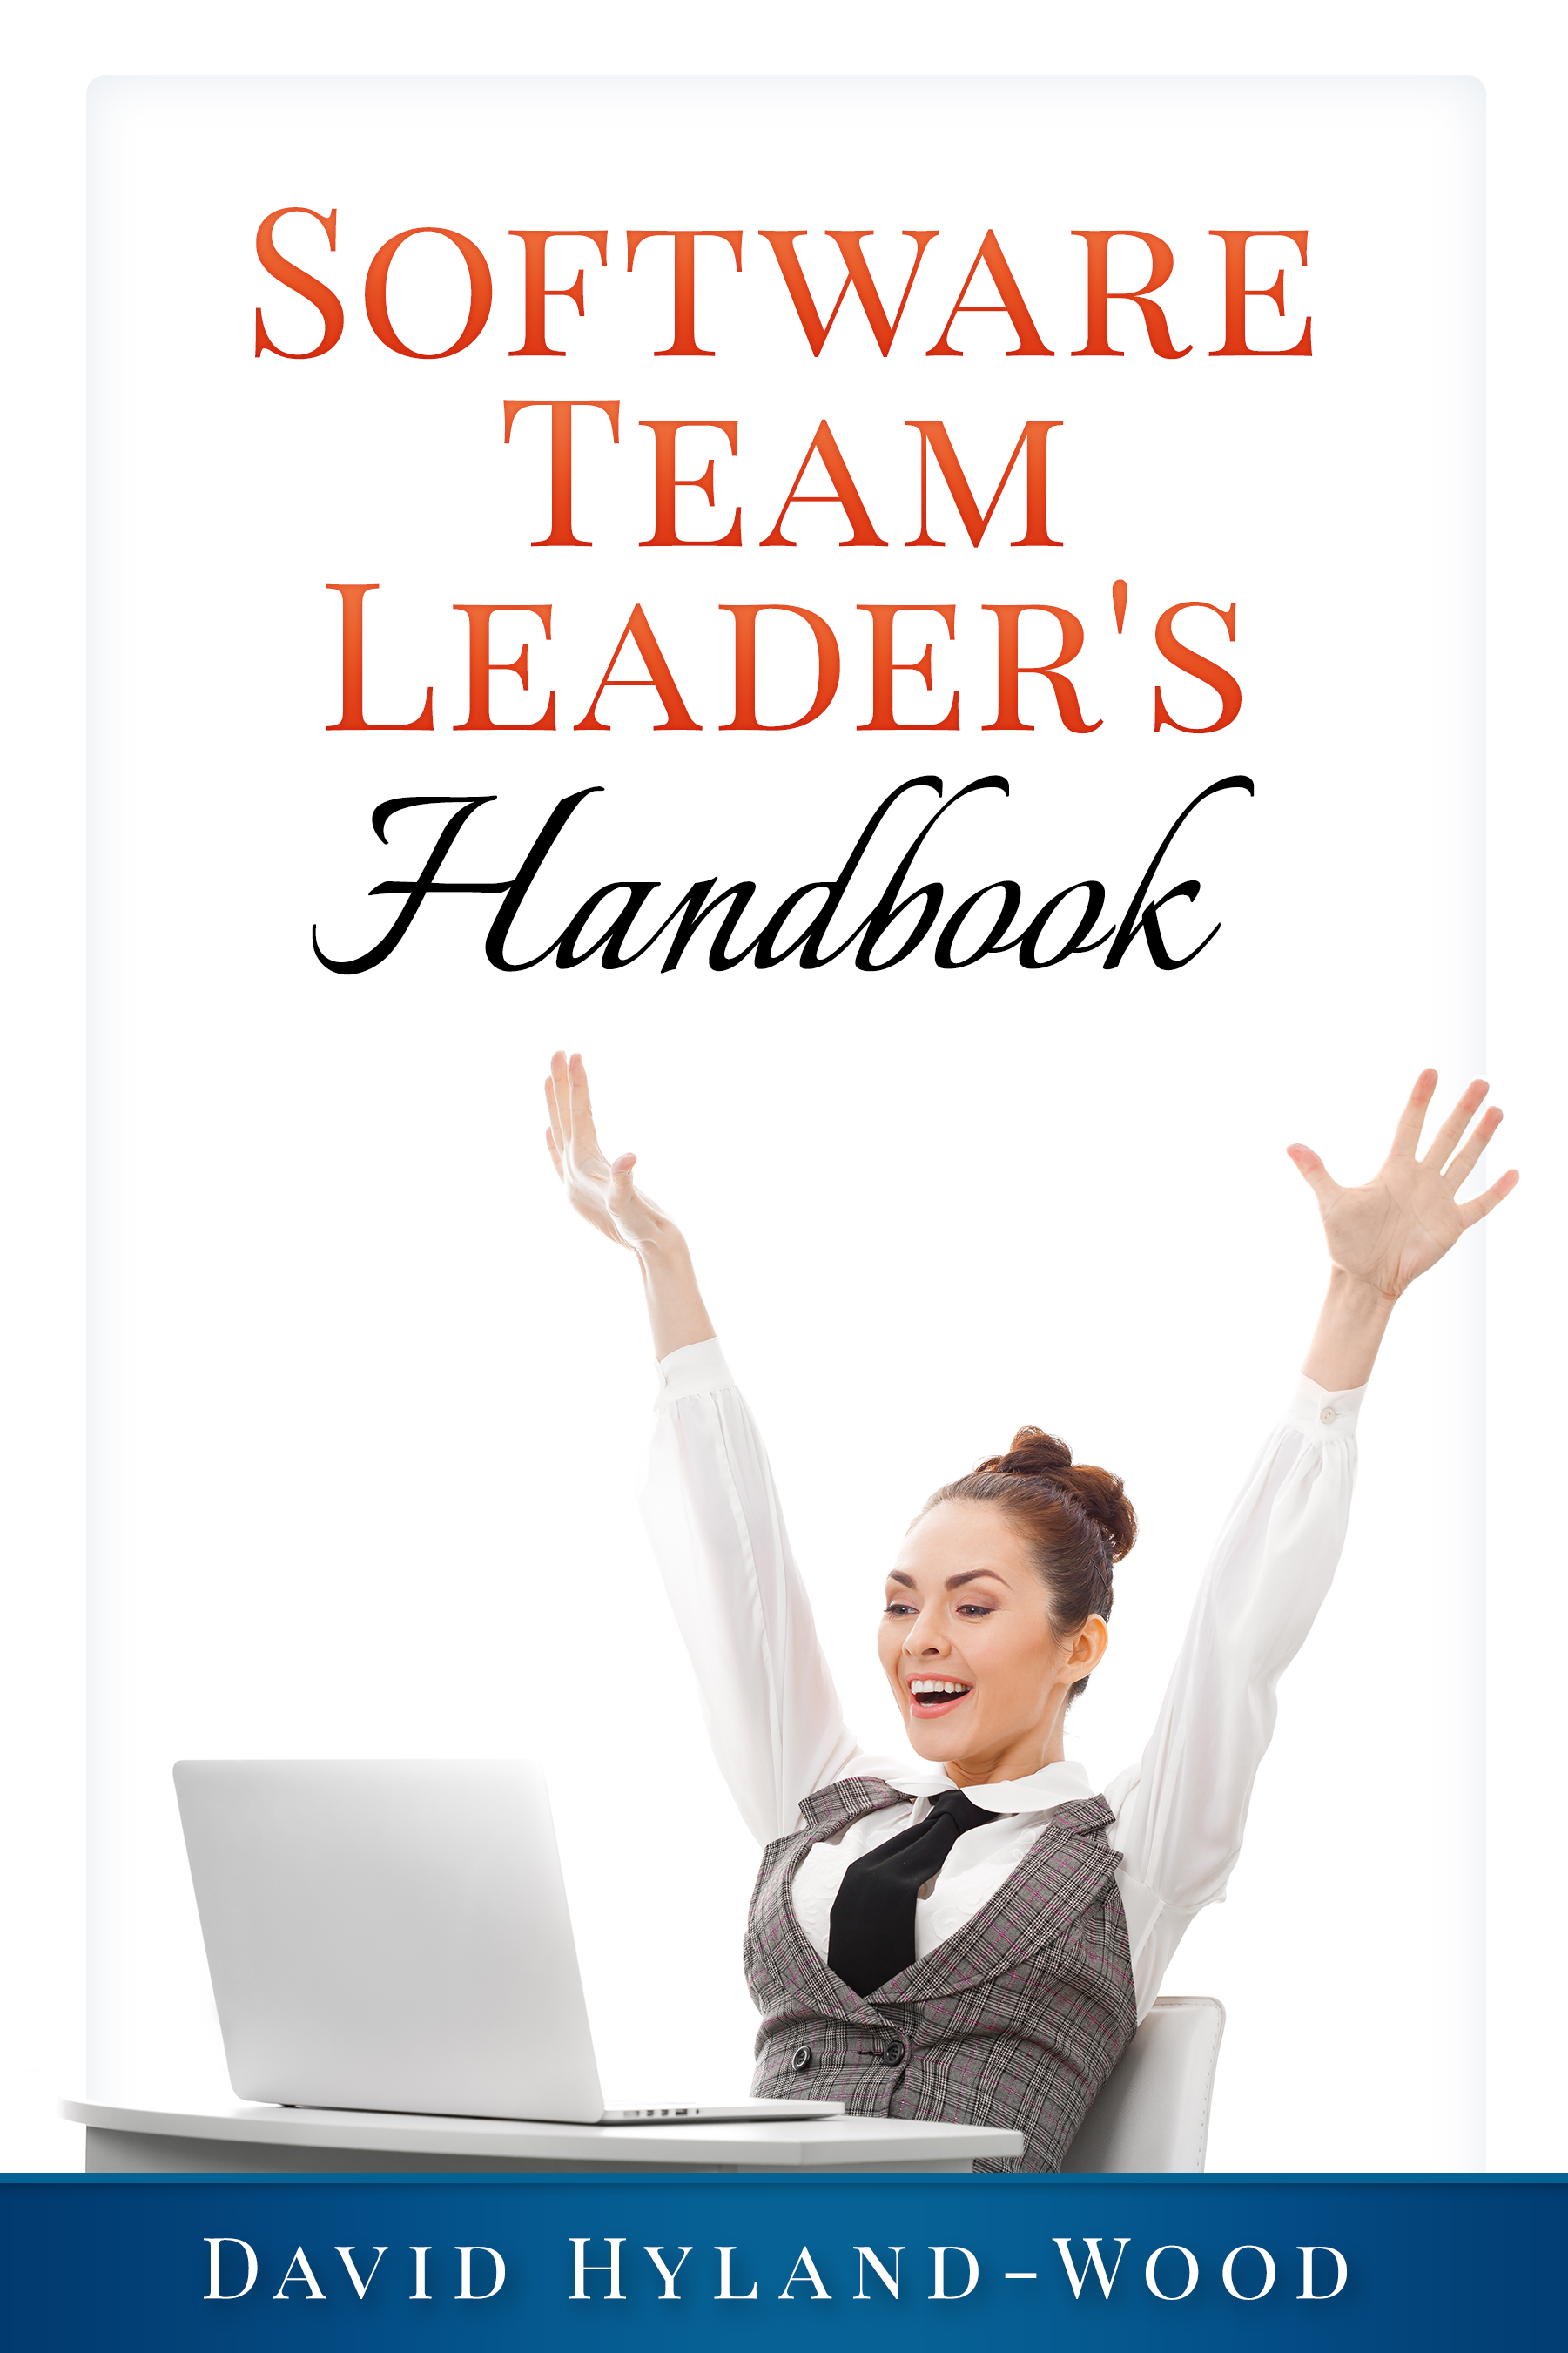
\includegraphics[width=1.00\textwidth]{front-back-matter/cover/STLH-DHW-front}
\end{center}
\end{figure}


\end{titlepage}

% Title Pages
%-------------------------------------------------------------------------------
\pagestyle{empty}

\begin{titlepage}
\vspace*{\fill}
\noindent
\textsc{Preview Edition, \today}

\vspace{5 mm}
\noindent
Copyright \textcopyright { }2016 by David P. Hyland-Wood

\vspace{5 mm}
\noindent
Permission is granted to copy, distribute and/or modify this document
under the terms of the GNU Free Documentation License, Version 1.3
or any later version published by the Free Software Foundation;
with the Invariant Sections being  "Acknowledgements", "Dedication",
and "History", no Front-Cover Texts, and no Back-Cover Texts.

\vspace{5 mm}
\noindent
\textbf{Library of Congress Cataloging in Publication Data} not yet registered.

\end{titlepage}

\pagestyle{empty}

%%%%%%%%%%%%%%%%%%%%%%%%%%%

\begin{titlepage}
\begin{center}

% Upper part of the page. The '~' is needed because \\
% only works if a paragraph has started.
%%\includegraphics[width=0.80\textwidth, frame]{cover/stlh_excerpt}~\\[1cm]

% Title
\HRule \\[0.4cm]
{ \Huge \bfseries Software Team Leaders Handbook \\[0.4cm] }
%\huge A subtitle would go here\\[0.5cm]
\HRule \\[1.5cm]

% Author
\noindent
\begin{minipage}{0.4\textwidth}
\begin{center} \large
\emph{by}\\
David P. Hyland-Wood
\end{center}
\end{minipage}%

\vfill

% Bottom of the page
{\large \today}

\end{center}
\end{titlepage}

% General definitions for all Chapters
%-------------------------------------------------------------------------------
% Define Page style for all chapters
\pagestyle{fancy}
% Delete the current section for header and footer
\fancyhf{}
% Set custom header
\lhead[]{\thepage}
\rhead[\thepage]{}
% Set arabic (1,2,3...) page numbering
\pagenumbering{arabic}
% Set double spacing for the text
\doublespacing

% Frontmatter
%-------------------------------------------------------------------------------
\frontmatter
% Frontmatter "chapters" have no chapter numbers, so use '\chapter*'.

%%%%%%%%%%%%%%%%%%%%%%% dedication.tex %%%%%%%%%%%%%%%%%%%%%%%%%%
% 
% dedication
% 
%%%%%%%%%%%%%%%%%%%%%%%%%%%%%%%%%%%%%%%%%%%%%%%%%%%%%%%%%

\thispagestyle{empty}
\begin{dedication}
This book is dedicated to the memory of David Carrington,\\*software engineering theorist, mentor and friend.
\end{dedication}
\newpage

%%\include{front-back-matter/acknowledgements}
%%\addcontentsline{toc}{chapter}{Acknowledgements} % Add to TOC

%%\include{front-back-matter/preface}
%%\addcontentsline{toc}{chapter}{Preface} % Add to TOC

% Table of Contents
%-------------------------------------------------------------------------------
\newpage
% Use dots between chapter name and page number
\renewcommand{\cftchapdotsep}{\cftdotsep}
% Include the ToC
\setcounter{tocdepth}{1} % Limit ToC depth to chapters and sections.
\tableofcontents

% If the chapter ends in an odd page, you may want to skip having the page
%  number in the empty page
\newpage
\thispagestyle{empty}

% Mainmatter
%-------------------------------------------------------------------------------
\mainmatter
% Mainmatter chapters have chapter numbers, so use '\chapter'.

%%%%%%%%%%%%%%%%%%%%%%%
%%%%%%%%%%%%%%%%%%%%%%%%%%%%%%%%%%%%%%%%%%%%%%%%%%
%
% Chapter:  Congratulations! Now What?
%
%%%%%%%%%%%%%%%%%%%%%%%%%%%%%%%%%%%%%%%%%%%%%%%%%%

\chapter{Congratulations! Now What?}

\begin{quote}
``Nothing in the world can take the place of persistence.  Talent will not; nothing is more common than unsuccessful men with talent. Genius will not; unrewarded genius is almost a proverb. Education will not; the world is full of educated derelicts. Persistence and determination alone are omnipotent.'' -- Calvin Coolidge
\end{quote}

Congratulations on your promotion to team leader! You have no doubt worked hard, and achieved a level of mastery of your craft. You probably know several programming languages reasonably well, and at least one particularly well.

Most team leaders are post-graduate professionals with some years of experience actively coding. You have probably been successful in writing and maintaining large software projects.

Regardless of how you arrived at this career milestone, you are to be commended that your organization saw fit to promote you. Congratulations!

But what are you expected to do? Has anyone explained your new role to you? If you are like many new team leaders, your organization may have expected you to figure that part out on your own. You are, after all, a professional problem solver. Surely figuring out your role is just another problem to solve.

You have probably heard that part of your role is to mentor others. Software engineers could often use more mentoring than they get the opportunity. Each of us is familiar with the desire to break a problem all by ourselves. There is no better way to learn the craft. But we also get stuck on hard problems, sometimes for long enough to slip schedules, or we explore a technical direction that yields massive technical debt. We could all use a good mentor when we find ourselves in trouble.

As a team leader, you will certainly need to adjust your schedule, and your own expectations. You will rarely have the freedom to code all day. You will be expected to talk to your team, and upper levels of management. You suddenly have responsibilities beyond code quality. You will need to interact more with people, as messy and complicated as they can be.

You might have a fear deep in your gut that you aren't ready to lead a team, or don't know how to handle people, or just a fear of the unknown. If you are as good as your organization thinks you are, you will take your responsibilities seriously. You will worry about your own abilities, and how to improve them.

You will already have become aware of the tendency of software projects to become much more messy than their original designs promised. You will have created beautifully simplistic data structures, only to see them become crowded with workarounds, and layered with hacks that you promised yourself would one day be refactored. Somehow, and quite suddenly, your personal responsibility for technical debt transcends your own mess. You now bear responsibility to understand and address the technical debt of your entire team. That can be an overwhelming burden.

Surely you can just code better. You can stay at work longer, and you can use your new-found skills to cover for others' newbie mistakes. You can fix it! Only your codebase isn't fixed, and you are tired. You cannot do the job of your entire team. You will know that you have gone too far down this path when you snap at a colleague in your tiredness, or give up so much of your personal time that you cease to feel like to have a life outside of work. Yielding to such temptation is common among new managers. You will find, sooner or later, that you cannot do it all.

How, then, to be a team leader? What does it mean to lead, anyway? What does leadership have to do with management? Is your new career path all about people and their problems, or will your still get to immerse yourself in software? Will you fall technically behind as you spread yourself too thin?

Where it can, this short book gives you answers. There are some. Where you will need to discover your own answers, it provides you with some new tools to help in the attempt.

Let's get the easy part out of the way: What does it mean to be a software team leader? Simply put, a software team leader must keep their team \textit{happy} and \textit{productive}. The following chapters will break those goals into manageable chunks, and describe them in more detail.

Keeping your team happy is a mnemonic for dealing with those soft, people-related, issues that tend to erode human contentedness. You may need to make a team from your team members. You will certainly need to keep that team orientation alive as times and staff change, and to balance how your team fits into the rest of your organization. Keeping people happy is mostly about defining and maintaining a group. That's what puts the team in your team leader title. You will need to become a sort of practical, empirical psychologist as you mature in your profession.

Keeping your team productive means to clear technical hurdles. That might mean writing code yourself, or helping others to do so. It might mean managing the software development methodology process used by your organization. It might even mean insulating your team from upper management so your team can get actual work done. Much of what this book discusses brings us back to people, even when the topic is technology.

\vspace{20pt}
\setlength{\fboxsep}{10pt}%
\shadowbox{
\begin{minipage}{11cm}
       \begin{center}
A software team leader must keep their team\\
\textit{happy} and \textit{productive}.
       \end{center}
       \end{minipage}
}

The next step is to realize that your fears, and your reactions to them, are not as specific to the software industry as you might believe. They are an integral part of being human. Most people feel when they are promoted that they are not fully ready for new responsibilities. Part of that feeling comes from our own emotional desires to minimize upheaval, what the keen American observer of human nature Eric Hoffer\index{Hoffer, Eric} called, ``the ordeal of change.'' It takes anyone time to adjust to new expectations, and new working conditions.

The poet T.S. Eliot\index{Eliot, T.S.} wasn't talking about software when he wrote his dark missive ``The Hollow Men''. He was pointing out the hopelessness that seeped into the European consciousness between the world wars. Every practicing software engineer, however, would recognize in these lines the frustration that occurs when a good design turns into imperfect running code:

\begin{verso}
Between the idea
And the reality
Between the motion
And the act
Falls the Shadow.
\end{verso}

Similarly, it has become common for software engineers to pass around an ancient aphorism originally attributed to the Greek physician Hippocrates\index{Hippocrates}: The life so short, the craft so long to learn. The thought is so poignant, so applicable to our everyday lives, that it has been copied, twisted, translated, and repeated for nearly two and a half millennia. The Romans loved it (as ``\textit{Ars longa, vita brevis}''), as did the ancient Jews. Geoffrey Chaucer\index{Chaucer, Geoffrey} included it in a short poem even though he left it out of the Canterbury Tales. It has appeared in modern literature up through and including rap music. Software engineers, perhaps more than most, would recognize their own struggles with the rest of Hippocrates' original sentence:

\begin{verso}
Life is short,
art long,
opportunity fleeting,
experience perilous,
decision difficult.
\end{verso}

I am not in a position to increase your lifespan, nor to change the fact that software is a never-ending opportunity to create. It is possible to provide some clues to how happy and productive software teams work. It is also possible to give you new tools to understand the dynamics of your team, both by introducing technically-oriented concepts, and people-oriented ones. Having those tools will make decision making easier.

\textbf{TODONEXT}: Everything you do will become a balancing act. Outline the various things to balance here!

\textbf{TODONEXT}: Outline the rest of the book here.


% If the chapter ends in an odd page, you may want to skip having the page
%  number in the empty page
\newpage
\thispagestyle{empty}

%%%%%%%%%%%%%%%%%%%%%%%%%%%%%%%%%%%%%%%%%%%%%%%%%%
%
% Chapter:  Software Engineering Theory for Team Leaders
%
%%%%%%%%%%%%%%%%%%%%%%%%%%%%%%%%%%%%%%%%%%%%%%%%%%

\label{ch:SETheory}
\chapter{Software Engineering Theory for Team Leaders}

\begin{quote}
``I believe that failure is less frequently attributable to either
insufficiency of means or impatience of labour than to a confused
understanding of the thing actually to be done.'' -- John Ruskin
\end{quote}


TODO:

\begin{itemize}
\item Three Pioneers: Brooks, Lehman, Glass
\item  Beck's Law: ``Maintenance is the normal state'', Extreme Programming Explained, pp. 135.
\begin{itemize}
	\item 60/60 Rule
	\item ``No Silver Bullet'' - Brooks again.
	\item Three historical fallacies (The fallacy of perfect knowledge, the fallacy of the big round ball and the fallacy of perfect execution) from thesis, Ch 2.
\end{itemize}
\item Brook's Law: ``Adding people to a late software project makes it later.''
\item Wood's Law:
\begin{itemize}
	\item Formal: ``A Lehman E-type software system is defined to be in maintenance failure when knowledge of its design and implementation is lost. Avoidance of maintenance failure therefore entails constant actions toward knowledge retention.''
	\item Informal: ``Losing knowledge of a software product causes maintenance failure.''
\end{itemize}
\end{itemize}

\textbf{TODONEXT}: ADD/FIX REFERENCES FROM THESIS.


Software engineering theories as developed both within and outside of academia would seem to have very little bearing upon the average software developer. The daily tools of a developer have certainly benefited from the decades, or even centuries, of mathematical research into logic, the physics, chemistry and electrical engineering used to construct their machinery, the computer science used to develop their operating system, device drivers, major algorithms, and languages, and even the interface design to be found in their application development environments. Software engineering, as a discipline, seems at best to be missing and at worst to be missing the point.

All of that changes when you become a team leader. Suddenly, software engineering theory has a lot to say about how you should pursue your daily tasks, and explains why you should do so.

\section{Three Pioneers: Brooks, Lehman, Glass}

Three computing pioneers attempted to define and collect ``laws'' of software evolution: Fred Brooks, Meir Lehman and Bob Glass. All three began their careers in industry, and all three ended as academics. It is instructive to review them briefly to see how they have stood the test of time, and to note the lessons they present for software team leaders.

Brooks defined four ``inherent properties'' of software based on his experience in the 1960s and 70s at IBM; complexity, conformity, changeability and invisibility \cite{Brooks-1987}. Software is \textit{complex} because programmers continue to define and use new levels of abstraction. This is the reverse procedure from the physical sciences, where practitioners have spent generations by doing the exact opposite. Software becomes more complex as it is forced to \textit{conform} to other systems, some of which are arbitrary (and arbitrarily complex) such as human social systems. Software evolves, it is \textit{changeable} throughout its life cycle. Finally, the geometric abstractions of software are mostly difficult or impossible to visualize. They are, to use Brooks' term, \textit{invisible}.

\textbf{TODO}: Add a label and reference to Appendix A
Lehman was the first to recognize that software evolves during its lifecycle [Lehman 1969]. Lehman's laws were initially based upon IBM's processes, then grew to encompass other sources. Lehman began to formulate his laws as early as 1974, then systematically sought refinements over more than twenty years \cite{Lehman-1997}.

Lehman specifically defined several types of software systems, but his laws only apply to ``evolving'' or E-type systems. The other types are those defined entirely by their specifications or procedures. Such systems are rare indeed. E-type systems are the most common type of software systems because they are those that model, and thus to need to track and respond to, changing real-world situations.

Lehman defined eight laws relating to E-type systems. Arguably the two most important echo Brooks: The Law of Continuing Change notes that a software project evolves continuously (Brooks' changeability) and the Law of Increasing Complexity suggests that a software project becomes less structured, or more complex, with time (Brooks' complexity and conformity). One may also consider Lehman's Law of Declining Quality, which states that a project's quality decreases during its lifecycle unless specific efforts are made to address it, although that would appear to be a consequence of increasing complexity.

Glass collected fifty-five ``facts'' of software engineering through the arduous process of surveying many different types of software development organizations in multiple countries over many years. He summarized his collected facts into four themes: complexity, poor estimation coupled with schedule pressure, a disconnect between software managers and technologists, and the delusion of hype. Glass concluded his multi-decadal study by saying, ``I would suggest that practitioners considering some tool, technique, method or methodology that is at odds with one or more of these facts should beware of serious pitfalls in what they are about to embark on.'' \cite{Glass-2003}, pp 187.

Applicability challenges to both Lehman and Glass were made during the 1990s, as Free/Libre/Open Source software models for development began to become commonplace. Glass even went so far as to state an opinion that Open Source software would not long survive in the market. In spite of this, the established laws of software engineering have continued to hold. Challenges today tend to be minor, and in very particular circumstances. All three models have been shown to hold across many domains, including Open Source development.

Of the three, it is Lehman that has long been recognized as the hallmark of the field. Perhaps the reason for this is simply that Lehman's laws are more detailed than Brooks', but easier to understand than the many facts put forth by Glass. That they all point in the same direction is comforting.

Lehman's laws are presented in more detail in Appendix \ref{app:LehmansLaws}.

One embarks on a career in software management without an understanding of Brooks' inherent properties, Lehman's Laws and Glass's Facts at their peril. The work of software engineering theorists can and does guide good managers toward the most effective management strategies. The remainder of this chapter will demonstrate exactly how this is so.


\section{Problems with the Building Metaphor}

\begin{quotation}
``Software is largely a service industry operating under the persistent but unfounded delusion that it is a manufacturing industry.'' -- Eric Raymond
\end{quotation}

TODO: A bit of history regarding design, development, and project management inherited from the other engineering disciplines.

TODO: Brooks recognized the limits of the building metaphor back in 1958, and wrote about its flaws through the end of his career. In his seminal 1986 essay ``No Silver Bullet'', he stated,

\begin{quotation}
The building metaphor has outlived its usefulness. It is time to change again. If, as I believe, the conceptual structures we construct today are too complicated to be accurately specified in advance, and complex to be built flawlessly, then we must take a radically different approach.
\end{quotation}

The approach that Brooks intended to take was to grow software, rather than build it. He specifically used evolutionary metaphors TODONEXT. Note how this presaged Scrum and Agile development.


\section{What We Mean by ``Maintenance''}

\begin{quote}
``Computer Science is the only discipline
in which we view adding a new wing to a building as being maintenance.'' -- Jim Horning
\end{quote}

TODO: Clean and fix.
Software has long been one of the most complex structures created by humans [Brooks 1987] and often the most expensive portion of engineered systems that include it, as foreseen in the 1970s by Barry Boehm [Boehm 1973]. Software maintenance is, often by far, the largest portion of the software lifecycle in terms of both cost and time [Glass 2003, pp. 115-124]. Software maintenance is thus critically important to the economics of modern engineered systems, from phones to cars, industrial furnaces to spacecraft. Yet, in spite of thirty years of study of the mechanisms and attributes of maintenance activities, there exist a number of significant open problems in the field. Software still becomes unmaintainable with time [Jones 2007] (known formally as ``maintenance failure'' and informally as ``bit-rotting'').

Maintenance failure is exacerbated by the rapid divergence of software systems and information about them. This divergence is typically a consequence of the loss of coupling between software components and system metadata [Van Doren 1997]. Many researchers have mapped the complicated relationships between software components and system metadata such as requirements, metrics and tests [e.g. Han 1994, Rugaber 2000, Welsh 1994a, Welsh 1994b]. In particular, the need for relational navigation of all of these entities has been recognized [Jarrott 2003]. The key to avoiding maintenance failure is maintaining knowledge of both the design and implementation of a software system.


\section{Confronting Challenges in Evolving Software}

Software maintenance has a checkered past.  It has been relatively ignored in favor of tools and techniques for software development.  Thus, a comment on the state of the field in 1983 (``Software maintenance has been almost always neglected'' [Parikh 1983, pp.8]) sounds much like a comment from 2003 (``... the computer science or software engineering curriculum that contains material on software maintenance is rare indeed.'' [Glass 2003, pp. 116]).  Software maintenance is so under-discussed and under-valued that it was possible for at least one author to publish a book on a software development methodology as late as 2000 without once mentioning maintenance. Recognizing that all may not proceed perfectly during initial development, the author of that methodology stated simply that, ``Corrections of errors or added materials are sent to the recipients of the original report with an explanatory letter.'' [Sandq 2000, page 235]  In spite of significant effort by software engineering theorists, such a blithe attitude toward maintenance is not uncommon, especially among consultants and developers able to pass maintenance tasks to others.

The earliest large-scale software systems were naturally reflections of their funding models.  Military and large corporations dominated funding and therefore development and use.  A smaller percentage of software systems developed in 2008 are developed for military and corporate users due to the existence of software products aimed at consumers.  Tools and techniques developed to assist development (such as packaging of code into libraries, use of version control systems, testing and logging systems, integrated development environments and higher-level languages) enabled a broader application of software.  Software was applied to a wide range of small and large business problems and even personal projects throughout the 1990s and 2000s.  By that time, software was no longer solely the purview of governments and large corporations.  Software maintenance became, and remains, everyone's problem.

There are provable costs to maintenance, such as the number of programmers, their equipment and facilities. Interestingly, the history of maintenance cost estimates shows that they have changed little in spite of radical changes in development tools and techniques. Maintenance today accounts for 40-80\% of a software project's total cost, with an average of 60\% [Glass 2003, pp. 115].  Earlier estimates were similar (and probably relied upon by Glass):  Shooman estimated 30-80\% in 1983 [Shooman 1983, pp. 16], in 1988 Yourdon said 50\% [Yourdon 1988, pp. 24], Pressman said 50-70\% [Pressman 1988, pp. 203], and Shere 60-70\% [Shere 1988, pp. 60].  Pressman went on to warn that, ``If your numbers indicate substantially less effort, it is probably an indication that much maintenance work is going unrecognized.'' [Pressman 1988, pp. 203]

Field deployment of software can lead to substantially worse maintenance scenarios, from high cost to loss of material or life.  A widely referenced U.S. Air Force project in 1976 was reported to cost \$75 per instruction to develop but \$4000 per instruction to maintain due to the inaccessibility of the components [Shooman 1983, pp. 484].  Field deployment still causes maintenance failures even though distributed computing techniques and the Internet now allow software to be remotely patched more easily. Field deployment exacerbated resolution of the infamous ``Year 2000 bug'' because many systems using two-digit year date handling routines were embedded in small devices such as handheld instruments and remote sensing kits [Jones 2006].  An extreme modern example is the onboard software update that caused a battery failure in the Mars Global Surveyor spacecraft in 2007 [Dunbar 2007].

Methodologies have been developed to address obvious failures in the management of software.  They have, almost exclusively, focused on development and not on maintenance.  Fred Brooks famously compared system development experiences of the 1970s to California's La Brea Tar Pits, where many dinosaurs struggled, died and became fossilized warnings to others: ``Large and small, massive and wiry, team after team has become entangled in the tar.  No one thing seems to cause the difficulty -- any particular paw can be pulled away.  But the accumulation of simultaneous and interacting factors brings slower and slower motion.'' [Brooks 1995, pp. 4]  Resulting systems were often functional, but also late, expensive and difficult to maintain.  Systematic efforts to find and fix each difficulty led to a series of software creation techniques, initially several forms of structured programming.  One of the goals of structured programming was to create systems that were readily modifiable or, in other words, maintainable [Martin 1985, pp. 4-5].

Unfortunately, structured programming, like other methodologies before and since, failed to address aspects of development that would later become critical for maintenance.  Jackson Structured Development (JSD), for example, started by describing the structure of each input and output data stream, not by performing analysis of a problem to be solved [Jackson 1983, pp. xii].  Most structured design methodologies emphasized the creation of maintainable systems based upon a combination of up-front design and documenting the code [Yourdon 1988, pp. 24-25].  These techniques are now seen as insufficient due to the constantly changing nature of requirements.  Perhaps they were known to be insufficient then, as well.  Yourdon said in the same work, ``Maintenance programming is a serious problem'' and had only experimental restructuring engines to suggest to those in need.  His work presumed that his readers were coding from scratch.

The role of documentation, either external or internal to a program, is primarily to assist maintenance efforts. Early and current researchers [e.g. from Boehm 1981 to Wiegers 2001] believe that documentation is the key to maintaining software systems, and regularly admonished practitioners for failing to keep it up to date.  Practitioners, in their turn, responded with an unwillingness to contribute to an inherently unreliable medium and a stubborn refusal to ignore schedule pressures. Documentation is generally out of date and incomplete at any stage of the software life cycle [Glass 2003, pp. 123]. Updating documentation is often treated as a chore, often not as an important part of a software deliverable. When documentation is created, it is most often created in isolation from the code itself.  Software without adequate documentation is thus created every day, in spite of the continued appearance of new development tools and methodologies. These factors collude to mortgage the future success of a software project and make maintenance progressively harder [Wiegers 2001].

Maintenance of structured code, like its successor object-orientation, was presumed to be easier, partially because the code would be easier to read and partially because programmers were encouraged to document their designs and decisions. Specific guidance was commonly given that in-code documentation was to record solely a developer's intent:  ``How [a] module works is not described.  This is best ascertained by \textit{actually reading the code}.'' (emphasis in original) [Martin 1985, pp. 54-57].  Some methodologies, such as Extreme Programming (XP), eschew guidance regarding comments at all and suggest that individual programmers should decide on a personal ``style'' [Beck 2005, pp. 69].  In spite of this, many managers and programmers have attempted to create commenting styles that described the code and were physically attached to it.  Examples include Brooks' self-documenting PL/1 code [Brooks 1995, pp. 173], Knuth's Literate Programming methodology [Knuth 1992], Larry Wall's Plain Old Documentation (POD), a mechanism for attaching documentation to scripts in the Perl language [Wall 1987], the Java programming language's Javadoc tool [Sun Microsystems 1994] and Dimitri van Heesch's Doxygen source code documentation generator [van Heesch 1997].

Lack of accurate documentation leads maintenance programmers to make changes without fully understanding their potential impact.  Software is known to become less reliable over time as successive enhancements during maintenance are made without a full and complete understanding of their impacts on other parts of the system (known as ``bad fix injection'').  As many as 20\% of defect repairs can result in injections of new defects, with the average amount around 7\% [Jones 1995].  Perhaps that value suggests progress; Brooks said in his 1975 classic, ``Fixing a defect has a substantial (20 to 50 percent) chance of introducing another.'' [Brooks 1995, pp. 242]

Roughly half of all working programmers are now engaged in maintaining existing software and that figure appears to be rising rapidly [Jones 2007].  One may view this trend as a measure of success for the software industry; systems that work are kept, not replaced.  It may be time to view software maintenance not as a problem at all, but as a consequence of the malleability of software-based systems.  Glass, a proponent of this idea, has suggested making maintenance a ``magnet'' for experienced programmers [Glass 2006].  That may be difficult to accomplish. Many of maintenance's woes may be laid at the feet of psychology, not engineering.  \textbf{TODO}: As the Vonnegut quote at the opening of Chapter I nicely summarizes, creative people seem to prefer acts of creation to those of maintenance, and that observation is not limited to software.  Learning to navigate someone else's code, using older languages or techniques and rigorously testing is not as fun or as glamorous as seeing a new feature appear in a GUI or seeing a complicated feature work for the first time.  Indeed, a common euphemism for ``programmer'' is ``developer'', not ``maintainer''.

A software system must be replaced when maintenance fails.  Replacement often requires reverse engineering of the original and modified requirements before a new system may be designed. Reverse engineering becomes necessary because the code and the information about the code have diverged to a degree that the best documentation for the system is the code itself. This is known as a "loss of coupling" between the software components and system metadata [Antoniol 2002].  Such a maintenance failure occurs as a direct result of (a) programmers creating new bugs via ``bad fix injection'', (b) breaking the documentation by failing to keep it up to date, and (c) failing to migrate away from aging or removed system dependencies.

\textbf{TODO}: Tie the fix to the above three problems into the last section, where Wood's Law is discussed. Use methodologies, and other processes, to specifically address these three problems!


\section{Mechanisms of Software Evolution}

Software that is maintained clearly changes, and generally becomes more complex, with time.  It may thus be said to ``evolve'' by the definition of that word.  May software be said to evolve in the sense of a Darwinesque evolutionary algorithm?  Meir Lehman suggested that the changes to IBM's OS/360 operating system resembled an evolutionary process [Lehman 1969] seven years before the biologist Richard Dawkins first proposed (in 1976) that many aspects of culture, including tools such as software programs, evolve in a Darwinesque manner, at least by analogy [Dawkins 1989].  Software programs, however, differ greatly from biological organisms.  An obvious and important difference is that the unit of modularity is not an ``individual'' [Nehaniv 2006].

Tools in general seem to evolve from dissatisfaction with their form (``form follows failure'') [Petroski 2006].  Software's form, as a medium for the creation of tools, seems to follow failure as well [Nehaniv 1997].  Both end users' and developers' dissatisfactions cause software to change [Reitz 2006].  There is, perhaps, a parallel to be drawn with biological evolution, where form follows competitive advantage.

Tight coupling of many software components, present in most systems, is known to inhibit evolvability of those systems [Reitz 2006].  The concept of loose coupling, where a relationship between two entities is made resilient to change by minimizing assumptions about the entities themselves, is a tenant of modern software architectures such as the World Wide Web.  The term ``loose coupling'' and its relationship to architectural resilience was borrowed from organizational studies [Weick 1976]. Similarly, the late binding of entity addressing can further reduce coupling [Fielding 2000].  The concepts of loose coupling and late binding are desired architectural properties for distributed software maintenance.

Their environment impacts biological systems continually, but that impact is limited to phenotype.  Only genetic changes, mutations, can be passed to offspring.  Software is not as fortunate.  It has been suggested that development tools, software documentation and even the state of the software itself impact the evolvability of a software system [Wernick 2006].

Mechanisms of software evolvability thus remain poorly understood.  Our immature understanding of how software systems evolve begs the question of how to avoid maintenance failure in existing systems and systems that will be created using existing techniques.  Theories of software evolution do not yet provide sufficient answers.

\section{Defining Software Maintenance}

The classic life cycle of software (i.e., the one software engineers adopted from our civil, mechanical and electrical brethren) places maintenance at the end of a series of linear development steps [Pressman 1988, pp. 5-7].  That makes sense for a bridge and it makes sense for a car.  It makes sense for computer hardware.  It even makes sense for some types of computer software, such as field deployed embedded systems with stable requirements.  There was much debate in the 1970s and 1980s whether it was appropriate for software in general.  At the heart of the debate was whether the addition of new features should be counted as ``maintenance''.  If a requirement changed, was it ``maintenance'' to change the implementing code?  What if a new requirement was added?  During those decades, at the dawn of software engineering research, software maintenance was variously seen as either a separate activity such redesign activities [e.g. Shooman 1983, pp. 16, 484] or not [e.g. Brooks 1995 pp. 242, Parikh 1983 pp. ix, Yourdon 1988 pp. 24].  The latter view eventually came to dominate, with some researchers expressing frustration with the definition but noting its common usage ([e.g. Martin 1983, pp. 4]).  The single fact that redesign activities are considered part of software maintenance separates software, conceptually and actually, from every other engineering discipline.

Redesign occurs because requirements change constantly.  Changing requirements were seen in the early days of software engineering as an unfortunate, and even avoidable, side effect of poor initial analysis. A study performed in 1976 reported that the top reasons for the high cost of software were ``user demands for enhancements'' and poor documentation [Shooman 1983 pp. 484-5].  If we adopt the perspective championed by Glass, however, we can see that user demands for enhancement are a feature, not a bug.  The total system cost of software may be high, but software allows us to create systems that simply would not be possible without it.  Consider what our systems would look like (and cost!) if they could only use hardware components.  Importantly, enterprises in a capitalist system exist within a competitive environment.  They must either adapt, or perish.  Other consumers of software, such as militaries, also compete.  The software that supports them must do the same.  Requirements are therefore bound to change constantly.

Researchers in the 1980s attempted to apply concepts of more mature engineering disciplines to software.  This thinking by analogy yielded some important insights, but eventually met with failure as the analogy was stretched beyond its limit.  Software, as we have already shown, is not analogous to hardware in terms of maintenance.  The classic production lifecycle was applied to software in spite of its inapplicability.  Pressman, for example, described maintenance as ``the reapplication of each of the preceding activities for existing software'' [Pressman 1988, pp. 6].  Development of software does not stop.  In other words, software development is not constrained by the mere fact of a delivery.  Delivery may, and usually does, occur many times in the course of a product.

Fully 60\% of maintenance activities relate to user-generated enhancements [Glass 2003, pp. 117].  Coupled with the fact that 60\% of software lifecycle costs relate to maintenance we get the so-called 60/60 Rule, one of the few proposed ``laws'' of software maintenance [Glass 2003, pp. 115-118].  The 60/60 Rule is shown in Figure 2-1.  Understanding changes to be made is a major activity during maintenance.  30\% of total maintenance time spent on understanding the existing product. [Glass 2003, pp. 115-124 and Shere 1988, pp. 61].  Martin [Martin 1983, pp.4] found that up to 80\% of maintenance activities relate to changing requirements.

\begin{figure}[htbp]
\begin{center}
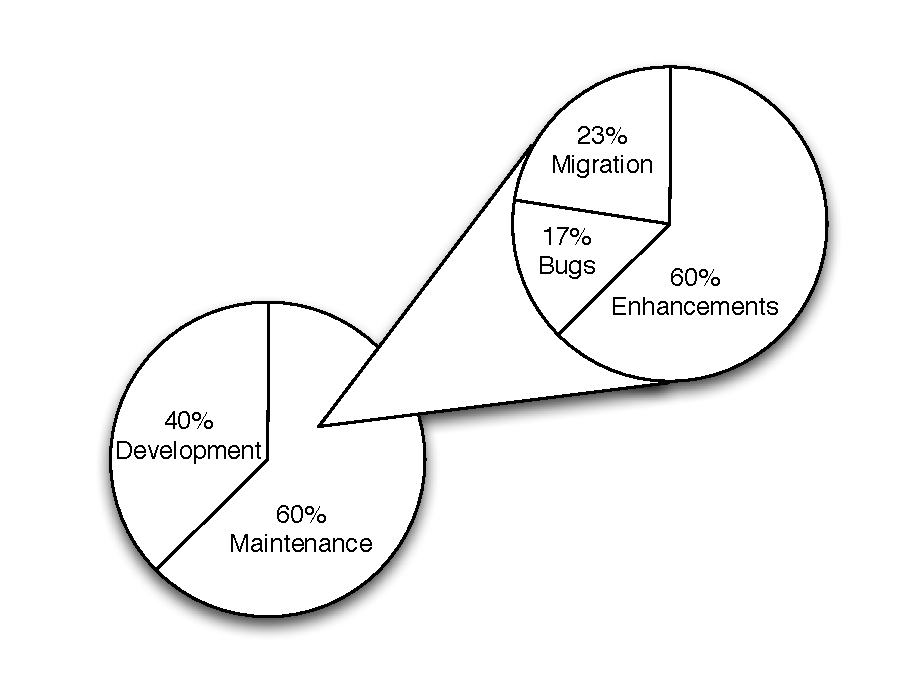
\includegraphics[width=1.00\textwidth]{theory/images/Figure2-1}
\caption{The 60/60 Rule of software maintenance costs.}
\label{fig:2.1}
\end{center}
\end{figure}

The 60/60 Rule should cause us to rethink the focus of software engineering research.  The tendency to address development activities may not yield the most impressive gains.  Boehm's early assertion [Boehm 1981] that proper software engineering discipline can reduce defects by up to 75\% may be true, and became the basis for much work toward development methodologies, but so what?  A good methodology may reduce bugs (17\% of the total maintenance effort), but not address migration or enhancement time or cost at all.

As a software project moves from development activities to maintenance ones, the amount of time spent attempting to understand, trace and redesign (what Glass calls ``undesign'') the code increases.  Testing and debugging time, often related to failures to comprehend a codebase, remain a major factor in spite of the existence of previous tests.  Table \ref{table:2.1} shows the breakdown of developer time spent during development and maintenance.

\begin{table}
    \centering
    \begin{tabular}{| l | c | c |}
    \hline
    \textbf{Task} & \textbf{Development} & \textbf{Maintenance} \\ \hline
    Understanding requirements & 20\% & 15\% \\ \hline
    Design/undesign & 20\% & 30\%  \\ \hline
    Implementing & 20\% & 20\%  \\ \hline
    Testing \& debugging & 40\% & 30\%  \\ \hline
    Documentation & & 5\%  \\ \hline
    \end{tabular}
    \caption[Table caption text]{Typical developer time spent during development and maintenance activities.}
    \label{table:2.1}
\end{table}


Maintainers were originally thought to be spending the bulk of their maintenance time creating enhancements because requirements were poorly captured.  See Figure TODO:2-2. It now seems that maintainers spend the bulk of their time changing requirements specifically because they can [Glass 2006].  Software, as Glass pointed out, is malleable.  Users, managers and investors generally see an economic benefit from modifying an existing system that almost meets their current requirements rather than creating a new one.

\textbf{TODO}: Expand here about the benefits of software: e.g. the number of MSL software updates compared with the number of hardware updates (zero). That just wouldn't be possible without software's malleable (and transmittable) properties.

Judged in that light, Boehm's statement that 20\% of defects account for 80\% of the work and 20\% of the modules account for 80\% of the defects [Selby 2007, pp. 3] would appear to be a benefit.  Poorly designed areas tend to cluster and may be refactored in one place.  New requirements, on the other hand, may or may not cluster, but directly leverage the malleability that is a central property of software.

\begin{figure}[htbp]
\begin{center}
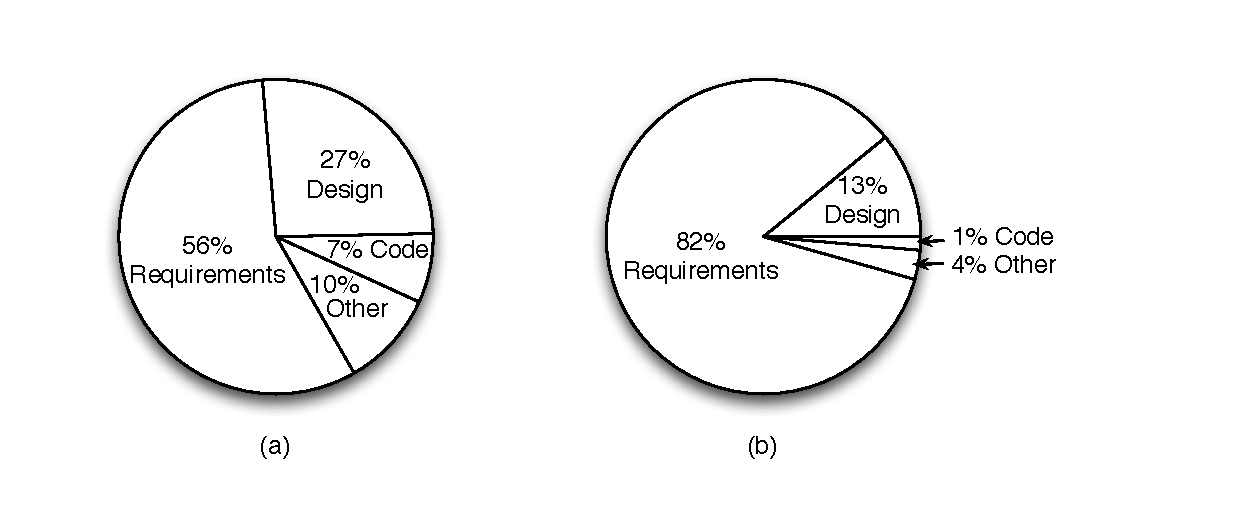
\includegraphics[width=1.00\textwidth]{theory/images/Figure2-2}
\caption{(a) The greatest number of bugs occur in requirements specification and design, (b) The greatest cost is incurred in correcting requirements bugs (After Martin 1983, Figure 12-3).}
\label{fig:2.2}
\end{center}
\end{figure}

Jones [Jones 2007] has refined the definition of software maintenance with a detailed delineation of twenty-three separate forms of modification.  However, he notes that each may be categorized as either defect repair or enhancement.  In my opinion, Jones does not change the definition of maintenance; he details it.

Acknowledging that redesign efforts are part of the software maintenance definition, we can still find obvious differences between creating enhancements and repairing defects.  Defect repairs, be they the result of bad fix injection, poor requirements gathering or failure to correctly implement a feature, do not require changes to the way the software is managed; the original expectation was one of defect-free operation already.  Enhancements, on the other hand, are expected to change the way the software operates, are documented and are tested.  Table \ref{table:2.2} summarizes the key differences.

\begin{table}
    \centering
    \begin{tabular}{| l | c | c |}
    \hline
    & \textbf{Enhancements} & \textbf{Defect Repairs} \\ \hline
    Funding Source & Clients & Developer \\ \hline
    Requirements & Formal & None  \\ \hline
    Specifications & Formal & None  \\ \hline
    Inspections & Formal & None  \\ \hline
    User documentation & Formal & None  \\ \hline
    New function testing & Formal & None  \\ \hline
    Regression testing & Formal & Minimal  \\
    \hline
    \end{tabular}
    \caption[Table caption text]{Typical differences between enhancements and defect repairs.}
    \label{table:2.2}
\end{table}

Clearly, some programmers will perform testing and update documentation (or even specifications and requirements) after repairing a defect, but the practice is all too uncommon.  Table \ref{table:2.2} should not be read as a criticism of programmer practices, but as recognition of trends in current practice.  Thus, the title of the table denotes ``typical'' differences between enhancements and defect repairs.

The Institute of Electrical and Electronic Engineers (IEEE) and the Association for Computing Machinery (ACM) have jointly defined software maintenance as, ``the process of modifying a software system or component after delivery to correct faults, improve performance or other attributes, or adapt to a changed environment'' [IEEE Standard Glossary 1990].  We note that the term ``delivery'' is ambiguous and suggests a classical view of the software lifecycle.  ``Delivery'' in the modern sense can constitute any number of production software releases or updates from conceptualization to retirement of a software product.


\section{Maintenance Failure}

A software product will eventually reach the end of its useful life.  The goal of software maintenance is to delay the end of life as long as possible.  Accordingly, the end of life for a software product is often a state known as ``maintenance failure''.  Maintenance failure eventually occurs in any software product that encodes requirements that remain extant.  Software products whose need is superseded (e.g. a product that calculates wholesale tax following the introduction of a comprehensive goods and services tax) may be removed from service prior to entering maintenance failure.

Maintenance failure may occur for several reasons.  The most common are that a product fails to adapt to changes in environment (such as hardware, operating system or necessary libraries) or it fails to adapt to new requirements.  The latter occurs when new requirements can no longer be added economically. [Brown 1980 pp. 279, Beck 2005 pp. 137]

Early researchers believed the solutions to maintenance failure were straightforward. After analyzing hundreds of software defects in the 1970s, pioneer researcher Barry Boehm said, ``if more time had been spent on validating the design... prior to coding many of the conceptual errors would not have been committed to code.'' [Selby 2007, pp. 1]  Note the connection to Figure TODO:2-2.  Boehm missed the connection from constantly changing requirements to constantly adding value by adapting to changing needs.

Shooman suggested in 1983 that poor documentation is the cause of maintenance failure: ``If the program is to be changed several times over a 10-year period, the documentation is more important than code... Obviously, in any sensible project we want both code and documentation.'' [Shooman 1983, pp. 486] ``It would be wise to pay, say, 10 percent more for the development of reliable software with proper documentation.  This will more than pay for itself in the long run through reduced maintenance and ease of redesign.'' [ibid. pp. 16]  ``The maintenance or modification costs will be strongly related to the quality of the documentation.'' [ibid. pp. 484] Shooman believed that the problems of software maintenance were understood and that the industry was well along the path toward implementing and fielding ``the solution''.  [ibid. pp. 19-20]  Unfortunately, the problems he identified were not solved by a combination of careful development practices and complete documentation.  His hopes for the future included, (a) improved languages and tools, (b) increased use of new development methods and (c) program proofs and automatic programming.  The first two have certainly happened and had an impact on productivity.  The latter has not happened on a large scale.  Although some progress has been recently made in the automated verification of general purpose code, we cannot yet judge how these new techniques will change our abilities to create software [Holzmann 2003].  Increased productivity in development has led to greater, not fewer maintenance challenges.

Yourdon postulated in 1988 that large software projects fail in development due to increasing complexities. ``A project involving up to 100,000 lines of code is sufficiently complex that neither the systems analyst nor the user is likely to have a clear understanding of exactly what the system is supposed to do, and even if there is a clear understanding, the user is likely to change his mind about some of the requirements.'' [Yourdon 1988, pp. 3].  This is the same phenomenon we reviewed earlier when discussing bad fix injection; bad fixes are inserted precisely because the developer does not understand the system.

TODO: Check first reference to Dunbar's Number.
There may be hard limits on our ability as human beings to understand complex systems and those limits are likely to be based in our physiology.  Dunbar's Number [Dunbar 1993] is a (mostly) accepted measure of the number of close interpersonal relationships that may be maintained by a human being.  This limit (roughly 150) is thought to be due to a physiological limitation of the human neocortex.  Human memory also has known limitations.  There are thus limitations to the complexity of a system comprehensible by humans.  One may certainly abstract from the details of a complex system to gain a general understanding or choose to understand a subcomponent in perfect detail.  The perfect understanding of all components coupled with a perfect understanding of the (often conflicting) intents of system users is simply not possible for very large software systems and arguably rare for smaller software systems.  The interpretation of requirements, documentation and code by multiple users, managers, analysts and programmers of a large software project, each according to their own imperfect understanding of what they are attempting to accomplish, merely adds to the complexity of the system.

Software systems and information about them diverge quickly in time, resulting in difficulties understanding and maintaining them.  This divergence is typically a consequence of the loss of coupling between software components and system metadata [Antoniol 2002].   Van Doren discusses an ``Evolution/Replacement Phase, in which the system is approaching or has reached insupportability. The software is no longer maintainable. It has become so 'entropic' or brittle that the cost and/or risk of significant change is too high, and/or the host hardware/software environment is obsolete. Even if none of these is true, the cost of implementing a new requirement is not tolerable because it takes too long under the maintenance environment. It is time to consider reengineering.'' [Van Doren 1997]  It is this type of maintenance failure that we strive most to prevent [Beck 2005, pp. 137].

None of these descriptions of maintenance failure address how we might migrate a software project back from the edge of maintainability; we are more likely to accept the inevitable, abandon the attempt and create a new one.  A primary goal for software team leaders should therefore be to avoid maintenance failure where possible and, where necessary, find means to (slowly, carefully, perhaps even painfully) recover a project's maintainability.  The solution is to lower local entropy and, like any closed system, that means we are required to put work into it.


\section{Three Historical Fallacies}

Much progress was made by the early 1980s in understanding the dynamics of software maintenance.  With a generation of large-scale system implementations behind them and software engineering research well underway, theorists believed that they understood what caused software to become unmaintainable.  Unfortunately, although researchers correctly captured the problems of software maintenance, their solutions were marred by three key fallacies, which we call \textit{The Fallacy of Perfect Knowledge}, \textit{The Fallacy of the Big Round Ball} and \textit{The Fallacy of Perfect Execution}.  As we show below, all three were the direct result of thinking by analogy about the practices of older engineering disciplines.


\subsection{The Fallacy of Perfect Knowledge}

The Fallacy of Perfect Knowledge states that it is possible to capture complete, non-conflicting requirements with sufficient attention to detail.  Requirements, even when agreed upon in detailed up-front design, will change.  It is impossible to know them all in advance.  Requirements gathered from more than one source can also result in inconsistencies.  Requirements may also mean different things to different people.  Differing interpretations may be due to perception, goals or language.  In order to create a general-purpose software maintenance methodology, we must accept and even embrace these ideas.


\subsection{The Fallacy of the Big Round Ball}

The Fallacy of the Big Round Ball states that requirements don't change appreciably after delivery or can be controlled.  Early researchers believed that if requirements could be fully understood before coding began, if the new structured programming techniques were rigidly adhered to, if new systems were documented fully and correctly, there would be no maintenance crisis.  Some academics and practitioners took note of the problem of post-delivery changes to requirements and labeled them evil; static requirements yielded more stable systems.  Some sought to limit a user's right to request changes (e.g., ``Reduce the need for change maintenance by planning for and controlling user enhancements'' -- one of a list of ``solutions to maintenance'' [Martin 1983, pp. 13]).  Unfortunately, such strict controls have the unintended side effect of making a software system less useful to its end users.  Such decisions, often based upon short-term economics, were greatly responsible for the alienation of information technology departments from their user bases in the 1990s and the subsequent development of smaller, often duplicate, software systems within business units during that period.


\subsection{The Fallacy of Perfect Execution}

The Fallacy of Perfect Execution states that it is possible to create flawless code with sufficient attention to detail.  We need to admit that arbitrary logic is hard to verify in the general case, and hard or impossible to fully test.  Drawing an analogy to the bricks and beams used in other construction-related activities, a researcher recently suggested that software is hard to verify because ``there are no good, predictable building blocks.  The elements out of which programs are constructed, statements, procedures, or objects cannot be composed in a predictable fashion'' [Dickerson 2006].  It is also hard to trace programmer intent, especially when requirements change or are inconsistently documented. Bugs will remain part of every software product shipped.

Admitting these three fallacies is tantamount to changing the way we think about the state of software at the end of development.  We can come to see delivered software as buggy, likely to change and with inaccurate documentation.  That insight, simple though it may be, encourages us to approach maintenance differently.  It encourages us to develop tools and techniques to incrementally refactor software implementations, requirements and documentation.


\section{Emerging Problems and Approaches}

Software currently in production was created using a great variety of techniques and procedures.  The software industry continues to struggle with this legacy and is expected to do so for the foreseeable future.  We therefore require a way to record information captured about these programs as they are maintained.  Failure to do that in a systematic manner leaves us where we are now; at the mercy of the memory of individual programmers assigned to a project.

\textbf:{TODO}: Look up relative amounts of procedural, functional, and OO code in production, and quote percentages.

The size of modern projects is increasing dramatically.  In 1988, Yourdon called 10M LOC ``utterly absurd'' [Yourdon 1988, pp. 2], but 2007 saw the Eclipse Foundation release its Europa coordinated project release with seventeen million source lines of code [http://www.linuxdevices.com/news/NS9334092346.html].  Similarly, an official Microsoft blog reported in 2006 that the company's popular Office suite for Macintosh computers measured thirty million source lines of code [http://blogs.msdn.com/macmojo/archive/2006/11/03/it-s-all-in-the-numbers.aspx].  The size of the maintenance domain is clearly increasing.

The key to maintaining complex software systems is to understand them. Victor Basili has said, ``Most software systems are complex, and modification requires a deep understanding of the functional and non-functional requirements, the mapping of functions to system components, and the interaction of components.'' [Basili 1982]  Many researchers have mapped the complicated relationships between domain knowledge, program components and system metadata such as requirements, metrics and tests [e.g. Rugaber 2000, Welsh 1994a].  Some have presaged this thesis in their interpretation of software development as a document-oriented process, and have recognized the importance of inter- and intra-document relationships in supporting traceability from requirements to implementation details [Han 1994, Welsh 1994b].

Research has variously focused on the relationship of program components [Wilde 1990], and the recovery of requirements traceability from source code [Coyle 2002, Antoniol 2002]. Unfortunately, the first is insufficient and the second, in its many forms, is ``not a trivial process'' [Han 1994].  We still require a way to capture and maintain our understanding of a code base that is broadly applicable.

The way we view software for maintenance, as a series of functions to be repaired and added to, is flawed for historical reasons.  The traditional view of a computer was a machine to be commanded via a series of instructions, those instructions being collected into functions.  The functions were collected into a hierarchy (a program), which led naturally to the concept of development structured around functions. [Jackson 1983, pp. 3-4].  We know today that many programs are not hierarchical, such as those designed with grid, object-oriented, message-oriented and resource-oriented architectures.  These more modern logical abstractions for describing computer programs are more Web-like.

\textbf{TODO}: Investigate ``Some problems of hierarchical thinking are investigated in Chapter III.'' Worth adding material here??

Software maintenance and software development, those two states of any software project, need to viewed as the continuum that they are.  Some people are already thinking this way.  So-called Agile methodologies are claimed to be in a constant state of maintenance.  Beck, one of the architects of Extreme Programming, put it this way:  ``Maintenance is really the normal state of an XP project.  You have to simultaneously produce new functionality, keep the existing system running, incorporate new people into the team, and bid farewell to members who move on.'' [Beck 2005, pp. 135-6]  Glass' view of maintenance as a positive outcome of successful projects fits nicely with Beck's model.

\textbf{TODO}: Add a callout box with ``Beck's Law'' here?

Karl Wiegers has gathered a series of principles for approaching requirements maintenance on existing systems [Wiegers 2001].  His collection importantly addresses not only broken code, but also the lack of correct documentation and understanding (of both code and requirements) so common in systems maintained over many years.  He suggests retaining the older documentation, even though it is knowingly out of date, and slowly bringing it to relevancy as one addresses each section of code.  This is a form of documentation refactorization.

A few researchers have attempted to combine the formal methods of software engineering with formal descriptions enabled by Semantic Web technologies (e.g. [Goth 2007]).  Tetlow, for example, claims that some of the benefits of formal methods have not been widely fielded because they are ``too abstract for the average developer''.   The benefit to Semantic Web techniques is that they are unreservedly formal, and yet may be used by developers ``in an exceptionally informal way'' [ibid.].  The W3C has drafted two documents to date dealing with ``Semantic Web-enabled software engineering''; a primer for developers of object-oriented software [Knublauch 2006] and another describing the use of formal ontologies for the description of software systems [Tetlow 2006]. 

\textbf{TODO}: INSERT REFERENCE TO MY OWN THESIS RESEARCH HERE, AND BEST-PAPER FROM IEEE. Note that ``This thesis builds upon Wieger's idea in Chapter VI but extend it in accordance with the metadata best practices for virtual information resources described in Chapter IV.'' and ``This thesis builds on some of the ideas of Semantic Web-enabled software engineering in Chapters VI and VII.''


\textbf{TODONEXT}: Wood's Law, and implications for software team leaders.
\section{Directions for Team Leaders}

A software project dies when it cannot recover from ``maintenance failure'', so focusing effort on maintenance activities that prolong the life of a project makes the most economic sense.

I might modestly call this Wood's Law:

\begin{itemize}
	\item Formal: ``A Lehman E-type software system is defined to be in maintenance failure when knowledge of its design and implementation is lost. Avoidance of maintenance failure therefore entails constant actions toward knowledge retention or knowledge re-acquisition.''
	\item Informal: ``Maintenance failure is caused by the loss of knowledge of a software product.''
\end{itemize}

\vspace{20pt}
\setlength{\fboxsep}{10pt}%
\shadowbox{
\begin{minipage}{11cm}
       \begin{center}
       \textbf{Wood's Law}\\
Maintenance failure is caused by the\\
loss of knowledge of a software product.
       \end{center}
       \end{minipage}
}

\textbf{TODO:} NOTE the lesson for team leaders in a callout box: Optimize for the activities you are mostly doing, not the ones with comparatively little value (such as creating perfect code).

\section{The Dark Art of Estimation}

\textbf{TODO:} Place in relation to old methodologies and their downfall. NOTE the ways that newer methodologies seek to estimate, not exactly schedule like the the old ones.



% If the chapter ends in an odd page, you may want to skip having the page
%  number in the empty page
\newpage
\thispagestyle{empty}

%%%%%%%%%%%%%%%%%%%%%%%%%%%%%%%%%%%%%%%%%%%%%%%%%%
%
% Chapter:  Leadership & Management
%
%%%%%%%%%%%%%%%%%%%%%%%%%%%%%%%%%%%%%%%%%%%%%%%%%%

\chapter{Leadership \& Management}

\begin{quote}
``Don't worry about people stealing your ideas. If your ideas are that good, you'll have to ram them down people's throats.'' -- Howard Aiken
\end{quote}

TODO: Tie back to Howard Aiken's quote somewhere later in the chapter (end of the leadership section?).


\section{The Face of Leadership}

It seems fair to say that most people who call themselves leaders or managers could not define what either term means.

The Oxford English Dictionary unhelpfully defines leadership as ``the act of leading a group of people or an organization'', and a leader as, ``the person who leads or commands a group, organization, or country.'' We obviously need to do better than looking to the canonical definition of our language.

Leadership is rightly approached with fear and trepidation, except by those few megalomaniacs who should not be given the responsibility. Management in its turn is often viewed as a ``black art'' by people expected to practice it, encompassing as it does a situationally dependent mix of tools, techniques, and applied psychology. It is difficult to find authoritative references. To anyone with a requirement to shepherd an organization however, it is most critical to define the differences and discover a personal path forward.

There are no lack of books purporting to demystify either leadership or management.  They abound.  The problem is that pop psychology is not the best guide to dealing with the complexities of real human societies.  Real human societies are the most complex thing ever built by people. Consider how contrary to human emotional tendencies are the workings of a democratic legislature and I think you will see what I mean.

It is often said that leaders are born, not made.  In contrast it is assumed that managers can be made.  There is no doubt that being charismatic helps a leader and that the procedures of management may be learned.  However, I think that one naturally goes hand-in-hand with the other and that a lack in one will illuminate weaknesses in the other.  It is my contention that both are learned skills and may only be assisted or hindered by one's natural gifts.

It is hard to find good books yet I think one can learn something from them.  I recommend reading a few biographies of leaders judged by history to have been superior.  George Patton\index{Patton, General George S.}'s ``War as I Knew it'' is a good start, as is Lee Iacocca\index{Iacocca, Lido Anthony ``Lee''}'s recollections of his experiences in the automobile industry. The collected letters of John and Abigail Adams\index{Adams, President John and Abigail} of US revolutionary fame round out a first collection. The most interesting collection of software-specific vignettes I know is \underline{Open Sources: Voices from the Open Source Revolution}\footnote{Available entirely online at \href{http://www.oreilly.com/openbook/opensources/book/index.html}{http://www.oreilly.com/openbook/opensources/book/index.html}}. You will assuredly want to ignore Paul Vixie's dated and facile description of software engineering in the 1990s, and instead focus on Richard Stallman's and Robert Young's descriptions of decision-making at the cusp of an era.

Leadership and management are often confused by those who would benefit most by clearly separating them.  Militaries, and often politicians, traditionally refer to all forms of oversight and control of people as ``leadership'' while the term ``management'' is more commonly used in business.  I make a finer distinction:  Leadership is the art of motivating people to operate as a team and management is the science of making those efforts effective.  Leadership is encouragement, coaching and psychology.  Management is your toolbox of procedures, time sheets, charts and graphs.  Put another way, leadership is about people and management is about organizations.

Leadership has one other critical aspect:  Accountability. The buck stops with the leader of an organization and that person must be both willing and able to make difficult decisions in a timely matter.  Failure to do so can lead to the failure of projects and even collapse of organizations.

\vspace{20pt}
\setlength{\fboxsep}{10pt}%
\shadowbox{
\begin{minipage}{11cm}
       \begin{center}
Leadership is the art of creating a team.\\
Management is the science of making those efforts effective.
       \end{center}
       \end{minipage}
}

The management consultant Peter F. Drucker\index{Drucker, Peter F.} had something very similar in mind when he said, ``Management is doing things right; leadership is doing the right things.''

Where Drucker and I differ is this: My definition of leadership stops when a team is formed. There is no mention of a \textit{mission}, nor where a leader is expected to lead. Who should say that it is the leader who chooses? This is very often not so. The mission may come from outside the team, as is commonplace in corporate software development, or even from the team members themselves. The latter is common in Open Source software projects. It is the mission that determines what Drucker's ``right things'' are.

The American leadership theorist James M. Burns\index{Burns, James M.} has perhaps the most influence on the academic debate when he separated ``transactional'' leadership from ``transformational'' leadership\cite{Burns-1978}. It is generally the former that I refer to as management, and the latter as leadership.

Software team members will generally express their dissatisfaction if the mission isn't worth the effort asked, or if it is simply wrongheaded. That is, no doubt, due to the generally higher degree of intelligence possessed of people who choose of their own free will to wrestle with machinery. The human species would have had a much more quiet history if all groups of people expressed dissatisfaction so readily, and so clearly.

A good leader will listen to the tenor of their group's conversations to constantly determine the level of satisfaction, and adjust their actions accordingly. Is this, then, not ``leading from behind''? If one is merely responding to the group's needs, in what sense can a leader be setting direction? Recall that maximizing a group's happiness is only one portion of a leader's responsibilities. The other, making the team productive, is equally important and is where the tools of management can help.


\section{A Word of Caution}

It has become your job to make a team from a group of disparate individuals. What, you might rightly ask, makes a team? The answer is surprisingly simple. Teams are made by establishing a shared identity.

Shared identity is a relatively straightforward concept to create. There are groups of people who get together because they share a common interest, such as dog breeding, or acting, or reading mysteries. There are groups based around religion, or ethnic identity, or even because they happen to share a small town. Software teams come nearly ready made in this sense, especially when they share the development and maintenance of a software product. A good leader can use the identity related to a product much more effectively than less meaningful identities, such as merely being an employee of a company.

However, and here is the warning, shared identity can also be created quickly and easily by convincing a group of people that they possess some form of special knowledge. That special knowledge separates them from everyone else. One often sees this in software development around conceptually difficult specialities, such as functional or logic programming, or in the mastery of a powerful yet esoteric programming language such as Smalltalk or Haskell.

Basing team identity on special knowledge is so often done because the idea is seductive. The temptation to create a bonded group quickly, and to harness the power that comes with it, is an easy way out. There is a dark side to such a decision. Basing a team on special knowledge, in the presence of a strong leader, is what defines a cult. Cultish behavior can and most often does result.

Taken to an extreme, cultish behavior leads to the excesses of a Stalin, or a Mao, or a Hitler, as well as to the formation of religious cults. On a smaller and more everyday scale, it can lead to a team that "believes their own press", and stops seeing the many clear indications that their products have critical flaws.

Cultish behavior in a business setting is how we get to the ``normalized deviancy'' discovered by Enron, and Volkswagen\footnote{For a particularly succinct description of Volkswagen's 2015 emissions scandal, see the  magazine article ``What Was Volkswagen Thinking?'' by Jerry Useem in the January-February 2016 issue of The Atlantic, \hyperlink{http://www.theatlantic.com/magazine/archive/2016/01/what-was-volkswagen-thinking/419127/}{http://www.theatlantic.com/magazine/archive/2016/01/what-was-volkswagen-thinking/419127/}.}.

The cure for cultish behavior and ``normalized deviancy'' is for both leaders and their teammates to constantly check themselves against outside opinion. If your actions seem odd to a domestic partner, or a close friend, they might very well be. Checking yourself and your team for the presence of cultish behavior is another in the long line of balancing acts. 

Leaders are not always thanked for doing the right thing, which makes leadership a lonely art. Many people do not wish to be told the objective truth, and would rather yield to the deep emotional comfort of a strong group identity. This is why we have strong cultural warnings about ``shooting the messenger", and why the second century CE Stoic philosopher (and Roman emperor) Marcus Aurelius warned us that a leader's job is, ``to do good and be damned.''\footnote{Marcus Aurelius, Meditations, book 7, section 36.}


\section{The Many Faces of Management}

According to my definition, there are many forms of management, but only one of leadership.  One may practice project management, personnel management, logistics management, etc.

One should not be insulted by being called a manager, nor feel unreasonably buoyed by being called a leader. The two are opposite sides of a coin, and cannot be separated.

Not all of the lessons of management are applicable to the software industry. Having a conception of the many faces of management can, however, be beneficial to the software team leader. It helps to place your own role in the greater schemes of human endeavor, and can give you ways to conceptualize the problems you will invariably encounter.


\subsection{Managerial Concepts}

Managers must understand their organization, and demonstrate that understanding.  We have all heard someone say, ``Everybody knows that it is wrong but management still makes us do it that way.''  This is a sign that those in charge don't know what is going on, don't listen to the people doing actual work, or (at best) haven't clearly communicated their reasoning to the rest of the organization.  All are critical errors in management.

Luckily, it is easy to correct such mistakes if one is willing to listen and learn.  The Total Quality Management (TQM) movement\footnote{TQM led directly to the adoption of the ISO 9000 series of management standards in 1987.} that began in the 1970s started with the simple realization that it is important to listen to assembly line workers' opinions.  They often discover ways to increase efficiency of operations. Unfortunately for those looking for a silver bullet, Total Quality ideas do not readily translate to other environments. They are particularly unsuited to non-procedural environments (such as research and development operations).

One of the best (and simple) ways to get to know an organization is still to talk to the people within it.  All of them. Regularly.  This is known as ``management by walking around'' (WBWA), also known by some as ``management by wandering around''. MBWA was a mainstay of the much-vaunted HP Way, used to great affect by Bill Hewlett and David Packard in their Silicon Valley company. MBWA is the best way, in my opinion, to understand small organizations, less than approximately 50 people - not by coincidence within the average size of a traditional human hunter-gatherer group.

Larger organizations are forced to implement progressively more hierarchy. Recent trends have been to flatten hierarchies as much as possible.  The degree of hierarchy is totally dependent on the goals of an organization.  Procedural organizations will generally require much more hierarchy than creative ones. Too much hierarchy decreases both creativity and productivity. Lack of necessary hierarchy overburdens management.

Managers of hierarchical organizations should still ``walk around'', if only to spot-check and get a feel for what is happening.  Hiding in an office will teach you exactly nothing about an organization.  Managers of hierarchies must meet regularly with those in charge of sections.  The amount of hierarchy must reflect the manager's ability to absorb section reports. In any case, organizational units should never exceed Dunbar's Number\footnote{British anthropologist Robin Dunbar theorized in 1992 that physical limitations of the human neocortex correlate to the number of stable social relationships that may be formed by an individual.} (approximately 150 individuals) without several hierarchical layers.

Managers should not be expected to know everything about their organizations, nor to be infallible!  In most organizations, a manager can afford the luxury of being a human being.  A possible exception exists for those in highly procedural environments where lives or property is at risk when an error occurs, such as a nuclear power station.  Even there, one must allow for human fallibility by building checks and balances into both social and technological systems.  The realization that humans routinely make mistakes is responsible for aircraft pilots having mandatory rest requirements, and for multiple nuclear weapons launch officers being required to agree before weapons activation.  In organizations where humans routinely operate while tired or under stress, procedural checks and balances must be followed.

Some managers follow a thumb rule of ``never asking a question for which you don't already know the answer".  This is a great idea if the manager is using the question as a training opportunity (to make the subject think about possible answers or to test the subject).  It is a horrible idea when the manager needs to determine the state of an organization and fails to ask critical questions.  In procedural environments, one might be expected to master a finite set of procedures over many years before being in charge.  It may be appropriate in those environments to ask only questions to which one already knows the answer.  Most organizations would be better managed if managers risked showing ignorance and asked legitimate questions.

Inexperienced managers often wish to appear more knowledgable than they are.  By failing to ask questions they ensure their continued ignorance and (in the end) fool nobody. The way to become an experienced manager is to learn your organization and the trade of management.  Ask questions. Respect will follow when you have earned it.

Good managers in all but the most mind-numbing of procedural organizations establish a culture of continuous learning. This can be in the form of training, encouragement of continued education, informal counseling, or some less formal form (such as simply reading books and leaving them around for others).

Training takes time.  It is also the best time that you can spend.  Constantly try to encourage people to the next level. Many managers ``build empires'' by protecting their knowledge. Instead, try training everyone to replace their superiors. You will be amazed at the results.  When you take the time to train people, they will notice that you care and their performance will rise.  Training is a very effective mechanism for team building, especially in organizations full of bright, capable people.

Software development organizations are some of the most fun to manage. They invariably consist of people more intelligent than the general population, and often have the advantage of a clearly defined shared goal. Software developers are renowned for their particular interests, hobbies, and personality types. Mastering the means of engaging with software developers as their own special category of people will pay off.


\subsection{Project Management}

Software team leaders may be wary of project management due to the explicit removal of the term ``project manager'' from the Scrum methodology. Project management was developed in a social framework of top-down control that seems to conflict directly with the team-oriented approaches of many software development frameworks. But the role played by a project manager is not entirely removed from those methodologies; they are present and simply distributed differently. It can therefore be useful to understand the term project management, and a bit of its history.

Project management is basically the application of applied economics to a project. Engineering as a discipline is also often described this way. In other words, almost anyone can get a job done given unlimited time and an unlimited budget.  Project management is a mechanism via which one ensures that a job may be successfully completed within a given budget.  Alternately, the tools of project management may be used to show that a job cannot be completed within the budget assigned.

Software teams generally struggle with the difficult task of estimating the amounts of time, effort, and budget are likely to be necessary to complete a project. There are good reasons for this, which are discussed in Chapter \ref{ch:SETheory}. Estimation, however difficult, remains a critical managerial task.

Project management can theoretically be as easy as choosing a methodology that suits your particular situation and learning how to apply it.  In mature disciplines, such as civil engineering, nobody discusses methodologies.  It would be foolish to ask a civil engineer which methodology they use to build a road.  There is only one, fine tuned over many decades to suit weather conditions, available road materials and other variables.  In immature disciplines, such as software engineering, methodologies abound. The number of competing methodologies is itself a sign of a rapidly changing industry.

The first software engineers borrowed the Waterfall methodology from older engineering fields. This is a wonderful way to track complex projects if the specification for the end product is not anticipated to change much during development. Stable requirements can, and do, occur in software projects, but it is an uncommon case. In response, software engineers developed new methodologies such as Rapid Application Development (RAD), the later Spiral RAD and, more recently, the so-called Agile methodologies such as Extreme Programming (XP) and Scrum.  Agile methodologies are appropriate for situations where it is difficult to determine a specification in advance (e.g. when no one group of people can adequately map available technology to known business problems), or when the specification is expected to change a great deal during development and maintenance.

Some of the great mistakes of project management are:
\begin{itemize}
\item Choosing the wrong methodology;
\item Assuming that a methodology will work for a given
        situation perfectly without modification;
\item Failing to adjust a methodology to local conditions;
\item Failing to adequately track a project's progress;
\item Over reliance on numbers or methodologies in place of
        an understanding of the project;
\item Failing to take adequate corrective action once a
        project is anticipated to be off schedule or budget.
\end{itemize}

All of these can be fatal errors and lead to a project's demise.  The last one may be viewed as a failure in leadership.

Traditional project managers master the use of conceptual tools to track a project's progress, such as Gantt and Pert charts.  These tools are generally taught in project management classes.  Gantt charts show task scheduling and Pert charts show task dependencies.  The two may be combined with task resource estimations to produce a critical path diagram which shows how fast a project may be completed in linear time.  All of these tools are critical to controlling a project managed with the Waterfall methodology.

In spite of their age, all project managers should learn and selectively apply these tools to their projects whenever requirements actually \textit{are} known up front, and expected to change slowly. Agile methodologies may eschew them, but it should be no surprise that modern Agile and Kanban tools, such as a Sprint Board, reintroduce (modified and time-scoped) tasking charts into software processes.

Some projects may have phases that are best handled by a combination of techniques. Knowing the available tools often keeps you from inventing your own. For example, you might be assigned to assist with the organization of an office move. Traditional project management tools and techniques then apply.

Another Waterfall concept is the formal specification. Traditional engineering teams produce functional (usage) and technical (implementation) specifications before beginning development.  Documentation is produced alongside development tasks as a parallel deliverable.  It may or may not be appropriate to develop specifications (or even documentation) for a software project, but any project manager worth the name should know how to produce them for those times when they are required.

The only thing that makes a ``good'' project manager is the ability to complete projects on time and on budget.  Under time and under budget is better.  Good project managers pride themselves on this ability. It is more challenging to do this for software projects than in any other field of engineering.

Good project managers posses one common trait:  They constantly think about their project.  Yes, this can interfere with social activities.  Good project managers worry, just a little bit, all the time.  This is because they are constantly aware of the state of their project and know what may go wrong.  They can calculate the impact of likely problems on schedule, cost and resourcing.  They prepare for the future before they future bites them (usually hard and in the middle of the night).  Good project managers thrive on the ``game'' of delivery.  Bad ones burn out.  Because of this worry, not everyone makes a good project manager.


\subsection{Logistics Management}

Plan ahead.  What will your team need next week, next month, and next year? Logistics management is an overly-fancy name for ensuring that your team has the materials they need to perform optimally.

Make certain that everyone has the tools and material necessary to do their jobs.  Plan to have a desk, chair, computer or other necessary equipment available on the \textit{first} day that a new employee joins. You never have a second opportunity to make a first impression.

The economic costs related to people, such as salaries, bonuses, holiday time, retirement savings, and other associated expenses, nearly always dominate the budget for a typical software organization. That means that spending should be aimed at keeping people productive.

\textbf{TODO}: Use an example budget
  for floor space, salaries, retirement, bonuses, equipment.
  Contrast with the budget for an aircraft carrier: even then
  people costs dominate.

A nice working environment will make people happy.  There is no reason to make people miserable.  Miserable people are not productive.  Slave labor is terribly inefficient, and centuries of brutal history have more than adequately demonstrated that it is simply a bad idea. Instead, relish your ability to create and maintain a positive and productive environment.

Failures of environment are the fault of the manager, even when resources are scare. Will you constantly complain that upper management does not give you the resources you want, or will you do well with what you have? Can you think of creative ways to better use what you can get? Software development organizations are generally better off economically than others. If you can't put emphasis on a good working environment, who can?

Thinking about logistics management can keep little things from getting in the way of productivity. This is especially important in software organizations, because programmers need time to just think. They should not be bothered by lack of toilet paper, running out of coffee or tea, or inexplicably losing access to basis services. Proper performance of logistics management can keep people from wasting valuable time, and from gossipy complaining -- that other bane of the happy workplace.


\section{Some Thoughts on Micromanagement}

Micromanagement is bound to be a temptation in environments where a (generally new) manager knows more about the way to do something than the person who should be doing the job. This is incredibly dangerous and is to be avoided at all costs.  No matter how tempting, \textbf{do not} micromanage.

If you really can do a job better \textit{and} the job is time critical \textit{and} there is no opportunity for training \textit{and} there is really no other choice after substantial thought, then simply assign the task to yourself.  Do not ``step in'' and perform a task while it was assigned to someone else. Doing so will seriously damage morale and is almost never worth the costs.  To make matters worse, you will be labelled a ``micromanager''. That is not a compliment.

A much better management style is to think ahead (as with all management tasks) and assign tasks to people based on their abilities.  Tend to assign tasks to people that are \textit{slightly} beyond their abilities, whenever possible.  When you encounter a situation which tempts you to micromanage, train the assigned person instead whenever possible, even if a schedule slips. Training always pays off in the long term.  The result will be high morale, a better team and a better organizational result.

Perhaps the final word should go to organizational consultant John Stocker, who sums up the dangers of micromanagement beautifully. Note how he equates micromanagement with other forms of bullying:

\begin{quotation}
``Authority -- when abused through micromanagement, intimidation, or verbal or nonverbal threats -- makes people shut down \& productivity ceases.''
\end{quotation}

There will be times to exert great control (e.g. over leave scheduling, budget, deliverables) and times to let the team rest.  Don't push hard all the time.  Be occasionally magnanimous.  Think hard every day about whether more or less control should be exerted today.  Once a team is established, back off and let them run with it.  If they do so, they are a team and you are a leader.


% If the chapter ends in an odd page, you may want to skip having the page
%  number in the empty page
\newpage
\thispagestyle{empty}




%%%%%%%%%%%%%%%%%%%%%%%%%%%%%%%%%%%%%%%%%%%%%%%%%%
%
% Chapter:  Managing People
%
%%%%%%%%%%%%%%%%%%%%%%%%%%%%%%%%%%%%%%%%%%%%%%%%%%


\chapter{Managing People}

\begin{quote}
``I don't believe in art. I believe in artists.'' -- Marcel Duchamp
\end{quote}

People are not resources. They are people. They have emotions, sick cats, girlfriends, boyfriends, ambitions and bad hair days. They are also the most amazing thing in the known universe. Treat people well and they will do amazing things.  Treat them poorly and you will get what you deserve.

Software engineers are generally smarter than average. They also have a job that makes them smarter over time. The constant solving of problems physically structures and refines the organization of the cerebral cortex. Of course, there are many different ways to be smart. It shouldn't surprise you when I say that software engineers tend toward a particular category of intelligence. They should be led accordingly.

Do not expect people to respect you because you wield power over them.  Respect is earned.  If you aren't getting any, you can either work harder to earn it or find other work. You earn respect by being a leader, not a manager.  You may gain a modicum of respect by being a competent manager, but it is not the same.

People generally distrust authority, especially when it is imposed on them.  Get off to a good start.  Make utterly sure that nobody is blocked by lack of simple resources.  Give people more benefits than they must have according to their contract.  Expect them to work only the hours they are contracted for.  If you have earned their respect, the results will surprise you every time.

Good managers isolate their team from external distractions. Good managers keep their teams informed.  This is another balancing act.

\textbf{TODO:} 
\begin{itemize}
\item be careful when communicating priorities; your team might take as fixed that which is variable, such as deadlines, features, stop shop items. 
\item Work prioritization both up as well as down!
\end{itemize}


One thousand ``well dones'' can be wiped out by one ``oh, damn''. Be forgiving of others but hold yourself to higher standards.


\section{Policies}

It is impossible to administer an organization of any size without policies.  Some examples might include the requirement to perform time reporting, a security requirement to restrict access to the Internet, or a definition of what separates a sick day from a leave day. It is important to have a clear and simple set of policies appropriate to your organization.  As the organization changes (as they all do, sometimes rapidly) policies must change to stay appropriate.  Too few policies is anarchy.  Too many policies stifles an organization's morale and creativity. Policy maintenance is a balancing act.

Enforcement of policies must be consistent!  If you take into account one person's personal circumstances, then take into account other's.

An effective leadership style is to praise in public and condemn in private. Humor may be used to softly remind otherwise good staff of deviance from policies.  Repeat offenders must be counseled immediately.  Consistent offenders must have their actions documented so there is no possibility of misunderstanding. They must be given every opportunity to conform and, if they don't, punishment (up to and including firing) must occur at a logical and expected pace.  Those violating safety, security or other policies deemed unforgivable (so-called ``zero tolerance'' policies) must have been clearly told beforehand and receive immediate punishment consistent with the rest of the organization.  Failure to be consistent will invariably undermine morale. Taking individual considerations into account is yet another balancing act.

It is impossible to administer an organization without meetings.  However, meetings should always be kept short, to the point and on target.  Regularly scheduled unproductive meetings kill productivity.  Short, productive meetings enhance communication. The effective use of MWBA can and should be used to limit both the number and length of meetings.


\section{People and Personalities}

\textbf{TODO}: Summarize, describe, and suggest (careful) uses for personality modeling. Note what you can get from it, and what you can't.

\textbf{TODO}: Use material from Dr. Ingrid de Meillon.


% If the chapter ends in an odd page, you may want to skip having the page
%  number in the empty page
\newpage
\thispagestyle{empty}

%%%%%%%%%%%%%%%%%%%%%%%%%%%%%%%%%%%%%%%%%%%%%%%%%%
%
% Chapter:  Understanding Business
%
%%%%%%%%%%%%%%%%%%%%%%%%%%%%%%%%%%%%%%%%%%%%%%%%%%


\chapter{Understanding Business}

\begin{quote}
``On two occasions I have been asked [by members of Parliament]: 'Pray, Mr. Babbage, if you put into the machine wrong figures, will the right answers come out?' I am not able rightly to apprehend the kind of confusion of ideas that could provoke such a question.'' -- Charles Babbage
\end{quote}


TODO: Introduction


\section{The Other 90\% of the Problem}

TODO: What Sales, Marketing, Administration, and HR care about, and how it will impact your life.


\section{Creating a Product that Sells}

TODO


\section{Interacting with Upper Management}

TODO: Understand their concerns, balance them with your own. Recognize that cliched misunderstandings of what is possible do occur, but are relatively rare; most conflicts with upper management are the result of competing priorities.


% If the chapter ends in an odd page, you may want to skip having the page
%  number in the empty page
\newpage
\thispagestyle{empty}

%%%%%%%%%%%%%%%%%%%%%%%%%%%%%%%%%%%%%%%%%%%%%%%%%%
%
% Chapter:  Fostering Innovation
%
%%%%%%%%%%%%%%%%%%%%%%%%%%%%%%%%%%%%%%%%%%%%%%%%%%


\chapter{Fostering Innovation}

\begin{quote}
``The reasonable man adapts himself to the world; the unreasonable one persists in trying to adapt the world to himself. Therefore all progress depends on the unreasonable man.'' -- George Bernard Shaw
\end{quote}


\section{The Adjacent Possible}

TODO


\section{Liquid Networks}

TODO: ``If an elderly but distinguished scientist says that something is possible, he is almost certainly right; but if he says that it is impossible, he is very probably wrong.'' -- Arthur C. Clarke

\section{Balancing Innovation and Happiness}

TODO


% If the chapter ends in an odd page, you may want to skip having the page
%  number in the empty page
\newpage
\thispagestyle{empty}






%%%%%%%%%%%%%%%%%%%%%%%%%%%%%%%%%%%%%%%%%%%%%%%%%%
%
% Chapter:  Management Scenarios
%
%%%%%%%%%%%%%%%%%%%%%%%%%%%%%%%%%%%%%%%%%%%%%%%%%%


\chapter{Management Scenarios}

\begin{quote}
``Faith is a wonderful thing, but doubt gets you an education.'' -- Wilson Mizner
\end{quote}

The following scenarios may be used as exercises for a team leader training class, or even as questions during job interviews. They are intended to make either reasonable discussion topics or written homework assignments.

All of these scenarios have occurred in my workplace during my career. You will need to think through the ramifications and decided for yourself how to keep your team happy and productive. Some possible approaches are provided, but none should be handled by simply choosing one of the provided answers. You should think about each scenario in the context of your own workplace.

It is often the case in real life that multiple approaches to a problem may be pursued in parallel. You should feel free to combine the approaches, and also to come up with your own answers.


\section{Trouble with Software}

\subsection{A Nasty Bug}

A seemingly unimportant bug is reported. Upon investigation, you determine that a major code re-architecture will be required to address the problem. What should you do?

Possible approaches:

\begin{enumerate}
\item Forget about it. If the bug is unimportant, why even consider a major change?
\item Deprioritize the bug so that it in unlikely to be discussed.
\item Think about it for a while in the hope of discovering a way around the limitation.
\item Discuss the limitation with your team, in the hope that one of them can discover a way around the limitation.
\item Inform upper management immediately, because you have discovered a limitation of your current system.
\end{enumerate}

How would your answer change if the bug was considered to be a ``stop ship'' issue for your next product release?


\subsection{Initial Setup}

A new programmer on your team is having trouble getting your product to compile on his computer. What should you do?

Possible approaches:

\begin{enumerate}
\item Don't worry about it. You expect each of your team members to overcome compilation problems on their own.
\item Leave it for a day, or a week. Eventually provide some help if absolutely necessary.
\item Allow them to work the problem for a short amount of time, then assist him.
\item Immediately assist the person by showing him how to overcome the problem.
\item Configure your team member's build environment by yourself without showing him how it was done.
\end{enumerate}


\section{Trouble with Estimation}

\subsection{The Black Art}

One of the programmers on your team consistently estimates that they can implement more than they actually can. What should you do?

Possible approaches:

\begin{enumerate}
\item Don't worry about it. Estimation doesn't really mean anything anyway. The product will get done when it is done.
\item Tell the programmer to estimate better.
\item Track the overestimations until you can spot the pattern, then apply a ``fix'' to each of the programmer's estimations.
\item Track the overestimations until you can spot the pattern, then counsel the programmer to help them estimate better.
\item Place the programmer on administrative review, and prepare to fire them if they don't improve.
\end{enumerate}


\subsection{Velocity of a Tortoise}

Your entire team is bad at estimating how long tasks will take to complete. What should you do?

Possible approaches:

\begin{enumerate}
\item Don't worry about it. Estimation doesn't really mean anything anyway. The product will get done when it is done.
\item Tell upper management that software estimation is impossible, so they should stop relying upon it.
\item Tell the team that they must get better at estimation.
\item Track the overestimations until you can spot the pattern for each programmer, then apply a ``fix'' to each of the programmer's estimations.
\item Track the overestimations until you can spot the overall pattern, then tell the team to adjust their estimates based on that information.
\item Investigate other software development methodologies to identify ways to improve your estimation.
\end{enumerate}


\section{Trouble with Facilities}

\subsection{Hot, Hot, Hot}

The air conditioning is off when you arrive at your office on a hot summer's day. Several people are already at work, and sweating profusely. You are the first senior person to arrive. What should you do?

Possible approaches:

\begin{enumerate}
\item Don't worry about it. One of the more senior managers will fix it when they get in.
\item Send a message to one of the more senior managers for their help or advice.
\item Investigate the air conditioning controls to see if you can fix it yourself.
\item Call a repair technician, and tell them to bill the company.
\item Give everyone the day off.
\end{enumerate}

How would your answer change if the only people affected are part of another team in a separate air conditioning zone to your own team?


\subsection{Hardware Failure}

You arrive at work to discover that your central revision control repository is offline. None of your team members can check in new work, but they can continue to work on their own local checkouts. What should you do?

Possible approaches:

\begin{enumerate}
\item Don't worry about it. One of the more senior managers will fix it when they get in.
\item Send a message to one of the more senior managers for their help or advice.
\item Investigate related physical machinery, logs, and software configuration to attempt to fix the problem yourself.
\item Call your systems administrator.
\item Tell your team to work locally until the problem is resolved. Assign other tasks to anyone who is blocked.
\item Give everyone the day off.
\end{enumerate}

How would your answer change if the only people affected are part of another team?

How was your approach similar to or different from your answer to the question above regarding air conditioning?


\section{Trouble with People}

This is the big one. People seem to spend their nights thinking up ways to stand out from the crowd. Not all of those ways are particularly helpful to maintaining harmony or being productive.

\subsection{A Hacker on the Team}

One of the programmers on your team is caught by you trying to crack the root password on the company's main file service. What should you do?

Possible approaches:

\begin{enumerate}
\item Don't worry about it. It is your system administrator's job to ensure the file service is unassailable.
\item Tell your systems administrator about the attempt.
\item Send a message to one of the more senior managers for their help or advice.
\item Tell everyone on your team.
\item Log into the file service if you have administrative access and stop the attempt.
\item Attempt to physically stop the perpetrator from continuing their actions.
\item Call the police and ask them to arrest the perpetrator.
\end{enumerate}

How would your answer change if you discovered that the hacker had been successful?

How would your answer change if instead of cracking the file service, the employee was instead caught reading the email of other employees?


\subsection{An Issue of Identity}

An employee arrives at work with a large pin on their shirt announcing ``I'M BISEXUAL'' in large letters followed by ``but don't tell anyone'' in nearly unreadably small letters. Some of your team members are accepting, some dismissive, and some decidedly hostile. Senior management has not yet noticed. Who will you tell, and what will you say?

Possible approaches:

\begin{enumerate}
\item Ignore it. Enforcing the organization's dress code is not your problem.
\item Don't worry about it. If it doesn't bother you, it shouldn't bother others.
\item Counsel the employee to take the pin off.
\item Counsel the team not to worry about it.
\item Tell your team that they should let their own religious or personal preferences dictate how they should treat the employee.
\item Tell your team that they should treat the employee like any any other team member, with respect and dignity.
\item Inform senior management that they should set or enforce a company-wide policy.
\end{enumerate}

How would your answer change if your were personally hostile to alternative sexualities?

How would your answer change if your organization had a policy strongly contrary to your personal opinion?


\subsection{Blissfully Unaware}

A happy and productive programmer on your team develops the annoying personal habit of loudly smacking chewing gum while concentrating. Your team members laugh about it at first, but then you begin to receive complaints. What should you do?

Possible approaches:

\begin{enumerate}
\item Don't worry about it. If it doesn't bother you, it shouldn't bother others.
\item Report the programmer to one of the more senior managers for their help or advice.
\item Move the programmer's desk away from other people.
\item Tell the disruptive employee to change their ways.
\item Place the programmer on administrative review, and prepare to fire them if they don't improve.
\end{enumerate}

How would your answer change if the disruptive employee was assigned to another team?

How would your answer change if the disruptive person was you, and you hadn't previously been conscious of it?


\subsection{A Simple Matter of Theft}

A fellow employee invites you to their apartment. Once there, you begin to recognize that the home is decorated with items belonging to your employer. Your host freely admits that they stole the materials, and presumes that you won't say anything. What should you do?

Possible approaches:

\begin{enumerate}
\item Ignore it, and pretend that you didn't notice.
\item Tell the employee that you won't say anything.
\item Tell the employee that they should return the stolen items, and that your won't say anything if they do.
\item Tell the employee that they need to tell senior management what they have done.
\item Inform senior management, and recommend that they show leniency.
\item Inform senior management, and recommend that the employee be fired.
\item Call the police and ask them to arrest the perpetrator.
\end{enumerate}

How would your answer change if you had a close personal relationship with the employee?


\section{How Bad Can It Get?}

I have experienced some decided oddities in my thirty-plus years of management. They are not common, but they can and do come out of a clear blue sky. Each of the following scenarios have also happened in my workplaces over those decades.

This is hardly a comprehensive list. The items may also serve as material for further discussion, team training, interview scenarios, or even just to point out the intrinsic humor of the human condition.

What would you do if you were faced with the following work days from hell?

\begin{enumerate}
\item An employee attempts suicide.
\item An employee is arrested while at work for domestic violence.
\item An engineering team resigns \textit{en mass} on the eve of a product launch.
\item An employee brings a goat to your office over a weekend, and leaves it there.
\item A proverbial disgruntled employee erases 80\% of the files on the company's server infrastructure overnight.
\item A fire, flood, or earthquake makes your office inaccessible.
\item Your office is robbed overnight.
\item An employee dies while at work.
\item An investor demands that your team be fired on the eve of a major holiday.
\item Your entire team arrives for work intoxicated.
\item An employee becomes addicted to an unaffordable substance, and steals important equipment from the company to support their habit.
\item Your boss leaves work with the spouse of another employee, and is subsequently chased at gunpoint by the cuckold across country for some months. Fortunately, he occasionally calls to see how you are faring.
\end{enumerate}

The last one is my personal favorite. Sometimes, all you can do is laugh.

% If the chapter ends in an odd page, you may want to skip having the page
%  number in the empty page
\newpage
\thispagestyle{empty}







% Backmatter
%-------------------------------------------------------------------------------

% Backmatter "chapters" have no chapter numbers, so use '\chapter*'.

%%%%%%%%%%%%%%%%%%%%%%preface.tex%%%%%%%%%%%%%%%%%%%%%%%%%%%
% 
% Lehman's Laws
% 
%%%%%%%%%%%%%%%%%%%%%%%%%%%%%%%%%%%%%%%%%%%%%%%%%%%%%%%

\begin{appendices}

\label{app:LehmansLaws}
\chapter{Lehman's Laws}

Lehman noted three types of software systems:

\begin{itemize}
\item Software systems defined entirely by their specification (S-type systems);
\item Software systems defined entirely by their procedures (P-type systems); and
\item Software systems written to perform some real-world activity, which must then evolve over time to match that activity (E-type systems).
\end{itemize}

Unsurprisingly, E-type systems form the vast bulk of software systems currently extant or planned. Lehman's Laws of software evolution apply to E-type systems.

\begin{enumerate}
\item \textbf{Continuing Change}: An E-type system must be continually adapted or it becomes progressively less satisfactory.
\item \textbf{Increasing Complexity}: As an E-type system evolves, its complexity increases unless work is done to maintain or reduce it.
\item \textbf{Self Regulation}: E-type system evolution processes are self-regulating with the distribution of product and process measures close to normal.
\item \textbf{Conservation of Organizational Stability (invariant work rate)}: The average effective global activity rate in an evolving E-type system is invariant over the product's lifetime.
\item \textbf{Conservation of Familiarity}: As an E-type system evolves, all associated with it, developers, sales personnel and users, for example, must maintain mastery of its content and behaviour to achieve satisfactory evolution. Excessive growth diminishes that mastery. Hence the average incremental growth remains invariant as the system evolves.
\item \textbf{Continuing Growth}: The functional content of an E-type system must be continually increased to maintain user satisfaction over its lifetime.
\item \textbf{Declining Quality}: The quality of an E-type system will appear to be declining unless it is rigorously maintained and adapted to operational environment changes.
\item \textbf{Feedback System}: E-type evolution processes constitute multi-level, multi-loop, multi-agent feedback systems and must be treated as such to achieve significant improvement over any reasonable base.
\end{enumerate}

Laws 1-3 were formulated in 1974, and have not changed since. Laws 4-5 were updated in 1978. Law 6 was updated in 1991. Laws 7-8 were updated in 1996. Rather amazingly, all eight laws are still considered to hold.

Lehman's Law's were defined in \cite{Lehman-1980a} and {Lehman-1980b}, and updated in \cite{Lehman-1997}. A modern modern validation may be found in \cite{Yu-2013}.

\end{appendices}

% If the chapter ends in an odd page, you may want to skip having the page
%  number in the empty page
\newpage
\thispagestyle{empty}


%%%%%%%%%%%%%%%%%%%%%%%%%%%%%%%%%%%%%%%%%%%%%%%%%%%%%%
% 
% References
% 
%%%%%%%%%%%%%%%%%%%%%%%%%%%%%%%%%%%%%%%%%%%%%%%%%%%%%%

\begin{thebibliography}{99.}%
\addcontentsline{toc}{chapter}{Bibliography} % Add to TOC

\bibitem{Brooks-1987} Brooks, F.P. (1987). No Silver Bullet: Essence and Accidents of Software Engineering, Computer, IEEE Computer Society Press, vol. 20, no. 4, pp. 10-19.

\bibitem{Brooks-1995} Frederick P. Brooks, Jr. The Mythical Man-Month. Addison-Wesley, Anniversary edition, 1995.

\bibitem{Burns-1978} J. M. Burns. Leadership. Harper and Row, New York, 1978.

\bibitem{Glass-2003} Robert L. Glass. Facts and Fallacies of Software Engineering. Pearson Education, Boston, MA, 2003.

\bibitem{Lehman-1980a} Meir M. Lehman (1980). ``Programs, Life Cycles, and Laws of Software Evolution''. Proc. IEEE, vol. 68, no. 9, pp. 1060-1076.

\bibitem{Lehman-1980b} Meir M. Lehman (1980). ``On Understanding Laws, Evolution, and Conservation in the Large-Program Life Cycle''. Journal of Systems and Software, vol. 1, pp. 213-221.

\bibitem{Lehman-1997} Meir M. Lehman, J. F. Ramil, P. D. Wernick, D. E. Perry, and W. M. Turski (1997). ``Metrics and laws of software evolution -- the nineties view''. Proc. 4th International Software Metrics Symposium (METRICS '97). pp. 20-32.

\bibitem{Yu-2013} Liguo Yu and Alok Mishra (Nov. 2013). ``An Empirical Study of Lehman's Law on Software Quality Evolution''. International Journal of Software and Informatics, vol. 7, no. 3, pp.469-481.


\end{thebibliography}
 % Added to TOC in the bibliography file

%%%%%%%%%%%%%%%%%%%%%%% acknowledgements.tex %%%%%%%%%%%%%%%%%%%%
% 
% About the Author
% 
%%%%%%%%%%%%%%%%%%%%%%%%%%%%%%%%%%%%%%%%%%%%%%%%%%%%%%%%

%\chapter*{About the Author}
\vspace*{\fill}
\begin{center}
\section*{\textbf{About the Author}}
\end{center}
\addcontentsline{toc}{chapter}{About the Author} % Add to TOC

David Hyland-Wood has been a ship navigator, deep sea salvage engineer, aerospace engineer, university researcher, lecturer, and software entrepreneur. He has contributed to the evolution of the World Wide Web since 1999, especially in the formation of standards and technologies for the Semantic Web. David holds a Ph.D. in Software Engineering from The University of Queensland, Australia; Aeronautical and Astronautical Engineer and M.S. in Astronautical Engineering from the U.S. Naval Postgraduate School and B.S. in Mechanical Engineering from the Virginia Military Institute. He is currently Director of Technology for Ephox, a software product company.

David blogs at \href{hyland-wood.org}{hyland-wood.org} and may be reached via Twitter \href{https://twitter.com/prototypo}{@prototypo}.
\vspace*{\fill}
% Added to TOC in the chapter file

\clearpage
\addcontentsline{toc}{chapter}{Index} % Add to TOC
\printindex
%-------------------------------------------------------------------------------

\end{document}

